\documentclass[conference]{joss-pretty}
\usepackage{natbib}

\title{Using a CubeSat Reference Architecture for Accelerated Model Development and Analysis (DRAFT)}

\keyword{[Model-Based Systems Engineering]}

\author{
Sean R. Kelly, Captain, United States Space Force \\
Air Force Institute of Technology\\
Wright-Patterson AFB, OH, USA
}

\abstract{
The domain of space systems engineering is transitioning to using Model-Based Systems Engineering tools, and Reference Architectures can assist with this transition. A Reference Architecture is a tool to capture prior knowledge and provide a starting point for teams to build from, facilitating rapid design, prototyping, and requirement verification and validation. This paper will describe a current effort to create a CubeSat Reference Architecture for use in a University setting, aiming to shorten the development time and improve model quality for teams going through an abbreviated design timeline. The current status of this CubeSat Reference Architecture will be described, and two new features will be highlighted in greater detail: built-in analysis using parametric diagrams, and traditional document generation. Future improvements for this Reference Architecture will also be discussed.
}

\begin{document}
\maketitle

\section{Introduction}
The CubeSat class of nanosatellites has lowered the barrier of entry to space and has rapidly gained popularity over recent years. The lower development cost, small form factor, and reuse of commercial off-the-shelf (COTS) components makes the CubeSat form factor an ideal platform for University teams, where budget and development time are extremely limited. In fact, many academic institutions have embraced this field for research and developed their own space programs. To successfully design a CubeSat system  in the graduate school time-frame, a Reference Architecture geared towards University CubeSat development would be helpful. A Reference Architecture would further speed up the development process by providing a template, capturing previous work and lessons learned from subject matter experts, and providing the framework to focus on the design rather than the fine details of modeling software. A Reference Architecture can also add functionality that student teams could use and improve over time, such as pre-built analysis functions and a library of components to choose from. This paper will discuss the need for a CubeSat Reference Architecture and explore features of one developed at the Air Force Institute of Technology (AFIT) for their space program. 

\subsection{Model-Based Systems Engineering}
The International Council on Systems Engineering (INCOSE) defines Systems Engineering as "\textit{An interdisciplinary approach and means to enable the realization of successful systems} \citep{INCOSEhandbook}." The system, comprised of a collection of hardware, software, people, facilities, and procedures, begins as a theoretical concept in the eyes of users or stakeholders, and from that idea, needs are defined, a system is developed and used operationally, and finally retired or disposed of \citep{Buede2016}. Systems Engineering is all about addressing this complete life cycle, and there are many strategies or techniques to accomplish this. The Department of Defense and NASA have traditionally used the "Systems Engineering Vee" model, a linear, document-based approach, but they are currently transitioning to the Model-Based Systems Engineering (MBSE) approach. 

Documents are the primary artifacts available to stakeholders \citep{Delligatti} in the traditional approach, including requirement and traceability matrices, interface documents, concept of operation documents, and other unique documents in a wide variety of formats. As systems become more complex, the traditional document-based approach becomes challenging to maintain. Each document is manually generated, so file management and version control are problematic. It is difficult to know for sure if a file is current or if it has been subsequently updated but located on some other file system or storage drive. Furthermore, any changes in one document, drawing, etc., must be also made in any other document that uses that same item. This system is prone to errors, inconsistencies, and difficulties maintaining an accurate representation of the entire system. MBSE provides a solution to these increasingly relevant problems. In MBSE, a system model represents the system and any information needed for documents can be found within this model. The model also makes it much easier to maintain consistency. If the modeler updates a component or interface in one area, it will be updated throughout the system as appropriate. Acquisition programs reviews will still require paper documents, but the necessary information for those can still be found within the system model. 

MBSE requires a modeling language, a modeling method, and a modeling tool \citep{Delligatti}. In this paper, those are respectively the Systems Modeling Language (SysML), the Object-Oriented Systems Engineering Method (OOSEM), and the Cameo Systems Modeler tool.

SysML is a standard modeling language that added systems engineering functionality to the Unified Modeling Language (UML) that has been used extensively in Software Engineering for decades \citep{Delligatti}. SysML provides a language, or the definitions and notations for nine different diagram types to describe a complex system, many of which will be used in this Reference Architecture. SysML is expressed graphically through those diagrams, listed in Figure \ref{fig:SysML Taxonomy}, to show various system viewpoints. For example, a Block Definition Diagram (bdd) expresses system structure, and an Activity Diagram can show specific system activities. Within "blocks", further detail can be expressed on an Internal Block Diagram (ibd). The SysML language is built into the modeling tool and allows for custom extensions if needed.

\begin{figure}
    \centering
    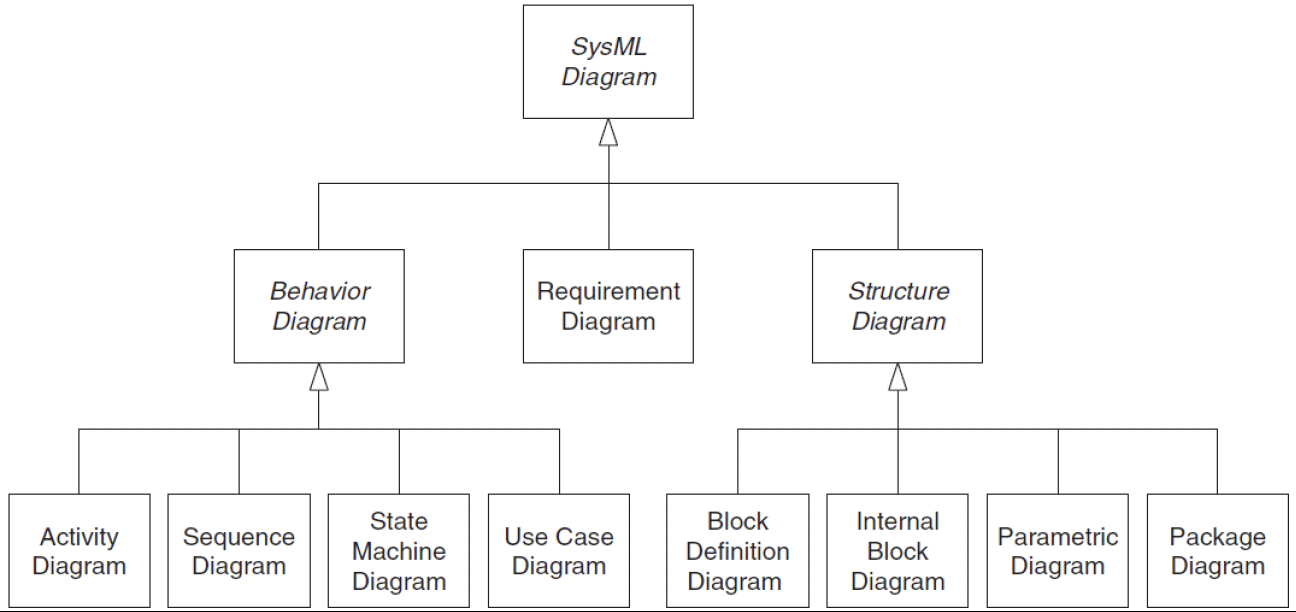
\includegraphics[width=\textwidth]{Figures/sysML taxonomy.png}
    \caption{SysML Taxonomy}
    \label{fig:SysML Taxonomy}
\end{figure}

The modeling method is the specific methodology used to ensure important design tasks have been accomplished and provides the general guidance, processes, or steps for the system design. This paper will focus on OOSEM, but there are other popular methods, such as the Weilkiens System Modeling (SYSMOD) method and the IBM Telelogic Harmony-SE method \citep{Delligatti}. 

OOSEM uses SysML in a top-down, model-based approach that leverages object-oriented concepts with traditional systems engineering methods to architect more flexible and extensible systems and can evolve with technology and changing requirements \citep{Estefan2008}. OOSEM was developed in part by Lockheed Martin Corporation as a method to capture and analyze requirements of complex systems, integrate with object-oriented software and hardware, and support system-level reuse and design evolution \citep{INCOSEhandbook}. 

OOSEM includes the following steps in an iterative fashion \cite{OMGwiki}, all of which are incorporated into the Reference Architecture.
\begin{enumerate}
\item{\textbf{Analyze Stakeholder Needs:} Capture the "as-is" system and mission enterprise and identify gaps or issues. The "as-is" depiction helps develop the "to-be" system, and the gaps or issues can help drive mission requirements for the new system. OOSEM frequently uses measures of effectiveness for the primary mission objectives identified in this step.}
\item{\textbf{Define System Requirements:} Once the "as-is" system is defined and produces Mission Requirements, the system is modeled as a "black box" in a Mission Enterprise model. For example, instead of going deep into subsystem-level detail on a CubeSat, the entire CubeSat will be a "black box" that interacts with ground stations, other satellites, and the environment. This "black box" model allows for system-level activity diagrams and use cases to show how the "to-be" system will support the mission enterprise. This step helps derive system-level functional, performance, and interface requirements.}
\item{\textbf{Define Logical Architecture:} A "logical" architecture is created that captures key functions in logical blocks, allowing for specific components to be chosen later in place of the logical depiction.}
\item{\textbf{Synthesize Candidate Allocated Architectures:} From the logical architecture, create potential physical instantiations using value properties and selected components. Each component at this stage is then traced to system requirements in table or matrix form.}
\item{\textbf{Optimize and Evaluate Alternatives:} Trade studies or other analysis is conducted at this step among the candidate architectures. Parametric diagrams within the model or integrating other tools can simulate system performance with the chosen components so alternative solutions can be compared.}
\item{\textbf{Validate and Verify System:} Once a candidate architecture has been chosen from the alternatives, the system needs to be validated and verified to ensure the requirements are being met and that stakeholder needs are satisfied. This step uses inspection, demonstration, analysis, and test activities to validate and verify the system.}
\end{enumerate}

Finally, the modeling tool is how the language and method work together. The modeling tool is a critical piece of software that maintains an underlying model of the system that can be used to display many different viewpoints or diagrams, depending on what is needed. The system model in a modeling tool is comprised of model elements and relationships between those elements, and from those, diagrams can be generated and displayed. When the source element or relationship is modified or deleted, that change gets carried out throughout the entire model, in any and all diagrams those elements or relationships appeared. This paper will focus on the Cameo Systems Modeler tool from No Magic Inc., but the process is tool-agnostic. Other tools are available on the market to accomplish the same goals with different user interfaces and feature sets.


\subsection{Reference Architectures}
Complex systems require a well-thought out architecture early on in the design process. The Department of Defense attempted to manage the “Enterprise-level Architectures” and “Solution Architectures” throughout the department by publishing the Department of Defense Architecture Framework (DoDAF). DoDAF defined an architecture as a “fundamental organization of a system embodied in its components, their relationships to each other and to its environment, and the principles governing its design and evolution over time \citep{DoDAF}.” This framework works well for major Defense Acquisition Programs, but small University teams that turn over every academic cycle have not been able to take advantage of this framework. 

A Reference Architecture can help alleviate that problem by consolidating subject matter expertise and previous relevant architectures into digestible models that system designers can benefit from when creating a Solution Architecture \citep{Cloutier2010}. The DoD saw the benefits of Reference Architectures and put out a Reference Architecture Description in 2010, describing them as \textit{“an authoritative source of information about a  specific subject area that guides and constrains the instantiations of multiple  architectures and solutions"} \citep{RADescription}. A Reference Architecture should be an "elaboration of company (enterprise) or consortium mission, vision, and strategy, facilitating a shared understanding about the current architecture and the vision on the future direction" \citep{Cloutier2010}. Furthermore, it should be continuously developed and improved over time as more teams use the architecture.

Finally, Reference Architectures should have at least the following elements:
\begin{enumerate}
\item{\textbf{Strategic Purpose:} Goals, objectives, and a specific purpose or problem to be addressed}
\item{\textbf{Principles:} High-level foundational statements of rules, culture, and values that drive  technical positions and patterns}
\item{\textbf{Technical Positions:} Technical guidance and standards that must be followed by solution  architectures (maybe data vocabulary/ data model)}
\item{\textbf{Patterns (Templates):} Generalized representations (e.g., Viewpoints, Views, Diagrams, Products, Artifacts) showing relationships between elements specified in the Technical Position}
\item{\textbf{Vocabulary:} acronyms, terms, definitions}
\end{enumerate}

Reference Architectures are being used in many industries, and at least one has been developed for CubeSats already. Kaslow, Ayres, et.al, as part of the International Council on Systems Engineering (INCOSE) Space Systems Working Group (SSWG), drafted a CubeSat Reference Model (CRM) to help promote and institutionalize the practice of MBSE for CubeSat development. Their CRM provides a reusable logical architecture for a generic CubeSat and provides a model to create a physical architecture from. (cite) The SSWG's CRM was useful for research, but did not meet the specific needs for AFIT students.

In summary, Reference Architectures can help systems engineers by providing a template, developed from years of experience, to aid in the systems engineering process. From the literature, it is clear that a Reference Architecture would be particularly useful for teams designing a CubeSat in a University setting, and this paper will address that need.

\subsection{Rapid Design Environment}
Between the compressed schedule, the distraction of other courses and projects, and the lack of modeling experience for most students, designing a satellite in graduate school is a challenge. At AFIT, the space vehicle design sequence lasts just nine months. Students start with a Mission Capabilities Document (MCD), outlining the stakeholders' required capabilities and design constraints, and from there, they're expected to derive mission, system, and subsystem-level requirements, design the physical architecture, simulate that design, and ultimately test physical hardware to verify the requirements. Throughout the process, they create traditional stakeholder documents, such as a Concept of Operations, Space Vehicle Requirements Document, etc., and build a system model from scratch. They must also demonstrate traceability throughout the model, from that original MCD through the tiers of requirements and to the physical components themselves. 

Clearly, developing brand new components within this short time period is not feasible, so Commercial Off the Shelf (COTS) components or previously developed components are used to accomplish their objectives. A component library within the Reference Architecture would aid this process so teams can reuse or improve previous model elements if applicable. Students could copy and paste existing component blocks and simulate their system using those blocks to quickly assess mission feasibility with the chosen parts. Additionally, the primary mission stakeholders would rather receive traditional documents instead of a complex system model, so the model should aid in that process. In the past, students would copy and paste diagram images or transcribe requirement text into other tools, but this Reference Architecture will automate this process to rapidly generate deliverable documentation.

In the University setting, the students generally come from a wide range of experience levels, with some having industry experience and others who have zero experience with satellites or with MBSE. Furthermore, students generally need to collaborate remotely due to their schedule demands. To address this, a cloud-based collaborative environment would be useful, and plenty of examples and guidance will aid the less experienced team members. Template tables and diagrams will be provided so students can focus more on the design choices instead of the details of model organization, structure, stereotypes, etc. In the end, a Reference Architecture should support rapidly designing, simulating, prototyping, and testing a system. 


\section{Developing a CubeSat Reference Architecture}
AFIT currently provides a model to assist students with the start of the design process through developing a Concept of Operations. This existing model was useful for capturing the Stakeholder Analysis and Mission Phases sections of the Reference Architecture, but teams quickly diverged from this model after the first course when support stopped. The primary goal of this Reference Architecture is to encourage the use of MBSE throughout the entire design sequence, all the way through the testing of hardware, so many more sections and capabilities were needed. Furthermore, the SSWG CRM papers were referenced for inspiration, and Sanford Friedenthal's diagrams in his book "Architecting Spacecraft with SysML" \citep{FriedenthalArchitectingSpacecraft} were also referenced. The primary source for equations, subsystem details, and mission activities was the textbook "Space Mission Engineering: The New SMAD" \citep{Wertz2011SpaceSMAD}.

The Reference Architecture opens with a splash page to show the organization of the model as shown in Figure \ref{fig:Model Organization}. It shows the top level package structure and includes hyperlinks to additional splash pages for each model section. This allows for intuitive navigation, instead of always digging into the containment tree to search for sections. The first package contains guidance for students, with a how-to guide and example diagrams for those newer to MBSE. 

\begin{figure}
    \centering
    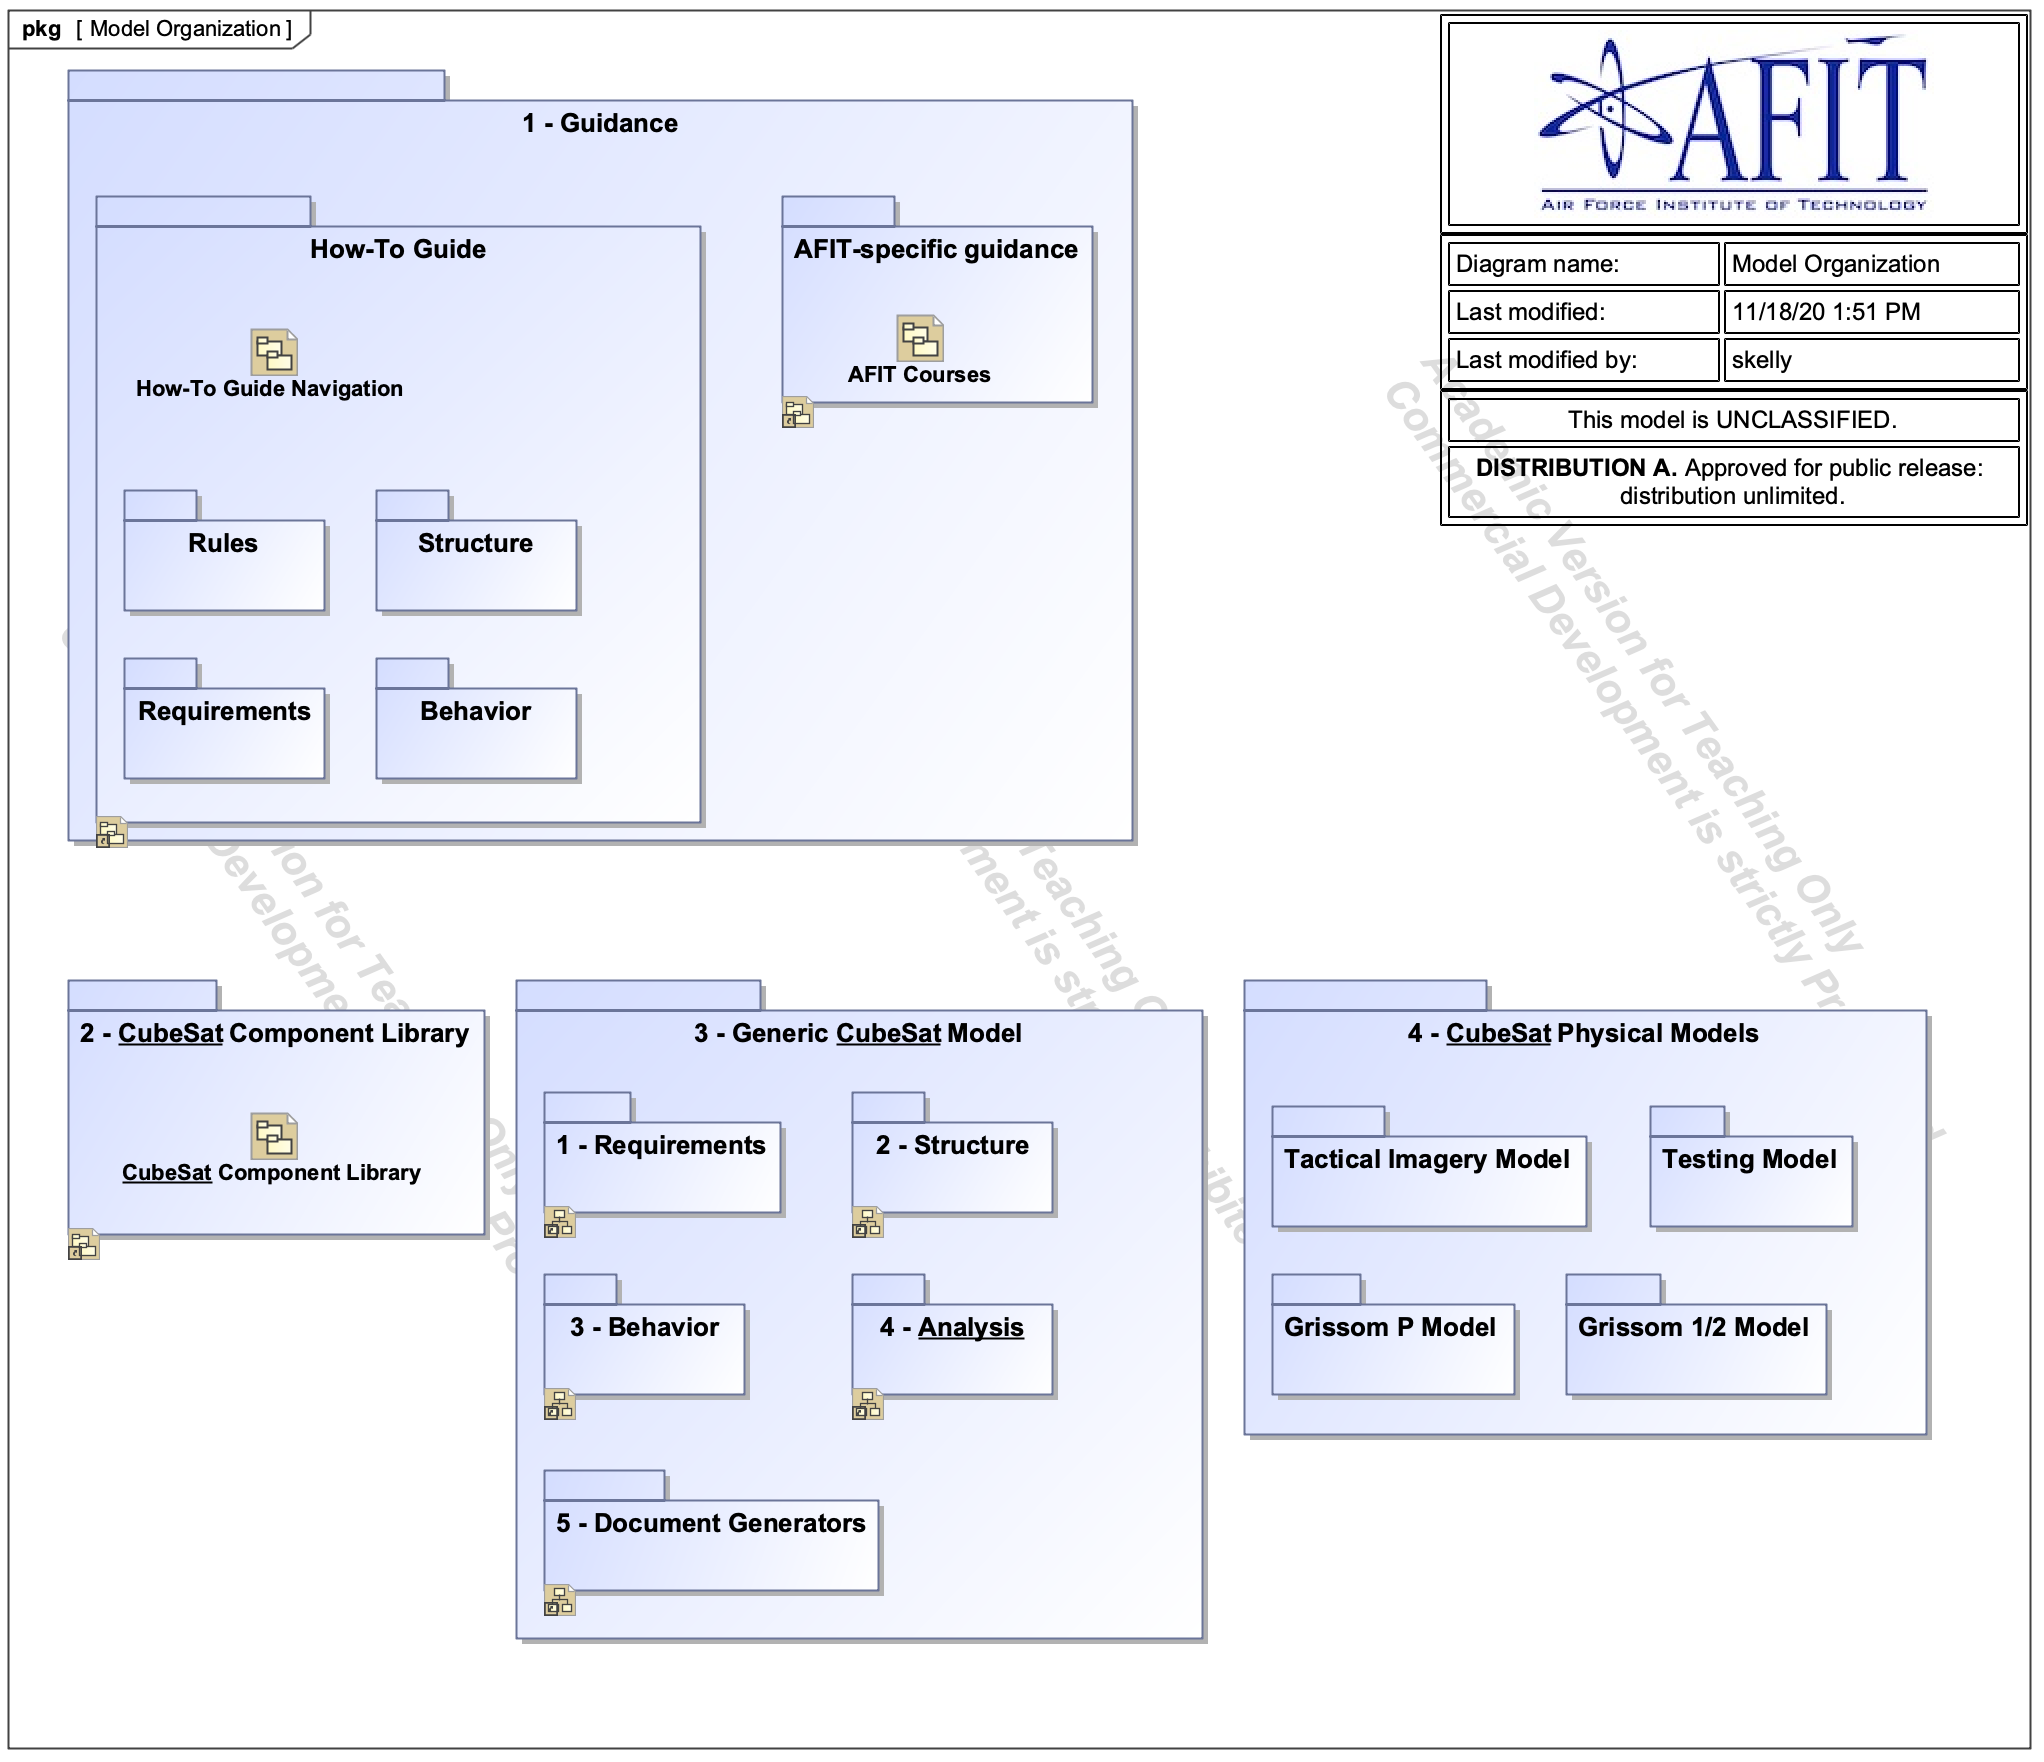
\includegraphics[width=\textwidth]{Figures/Model Organization.png}
    \caption{Model Organization}
    \label{fig:Model Organization}
\end{figure}

The Component Library is a new feature inspired by an AFIT-developed Small Unmanned Aircraft System (SUAS) Reference Architecture \citep{Jacques2019}. This feature is still a work in progress, but the goal is to have a library of components for each subsystem that can be reused in new models for rapid prototyping. For example, if an engineer wants to quickly test how different antenna options affect the RF link analysis, they can grab the antenna blocks in the component library, each having value properties that affect the calculations in the Analysis section of the model. The Component Library structure is shown in Figure \ref{fig:Component Library Organization}. Each subsystem has starter components contained within the respective packages, and the intent is for this library to be updated as new CubeSat designs are created using the Reference Architecture. 

\begin{figure}
    \centering
    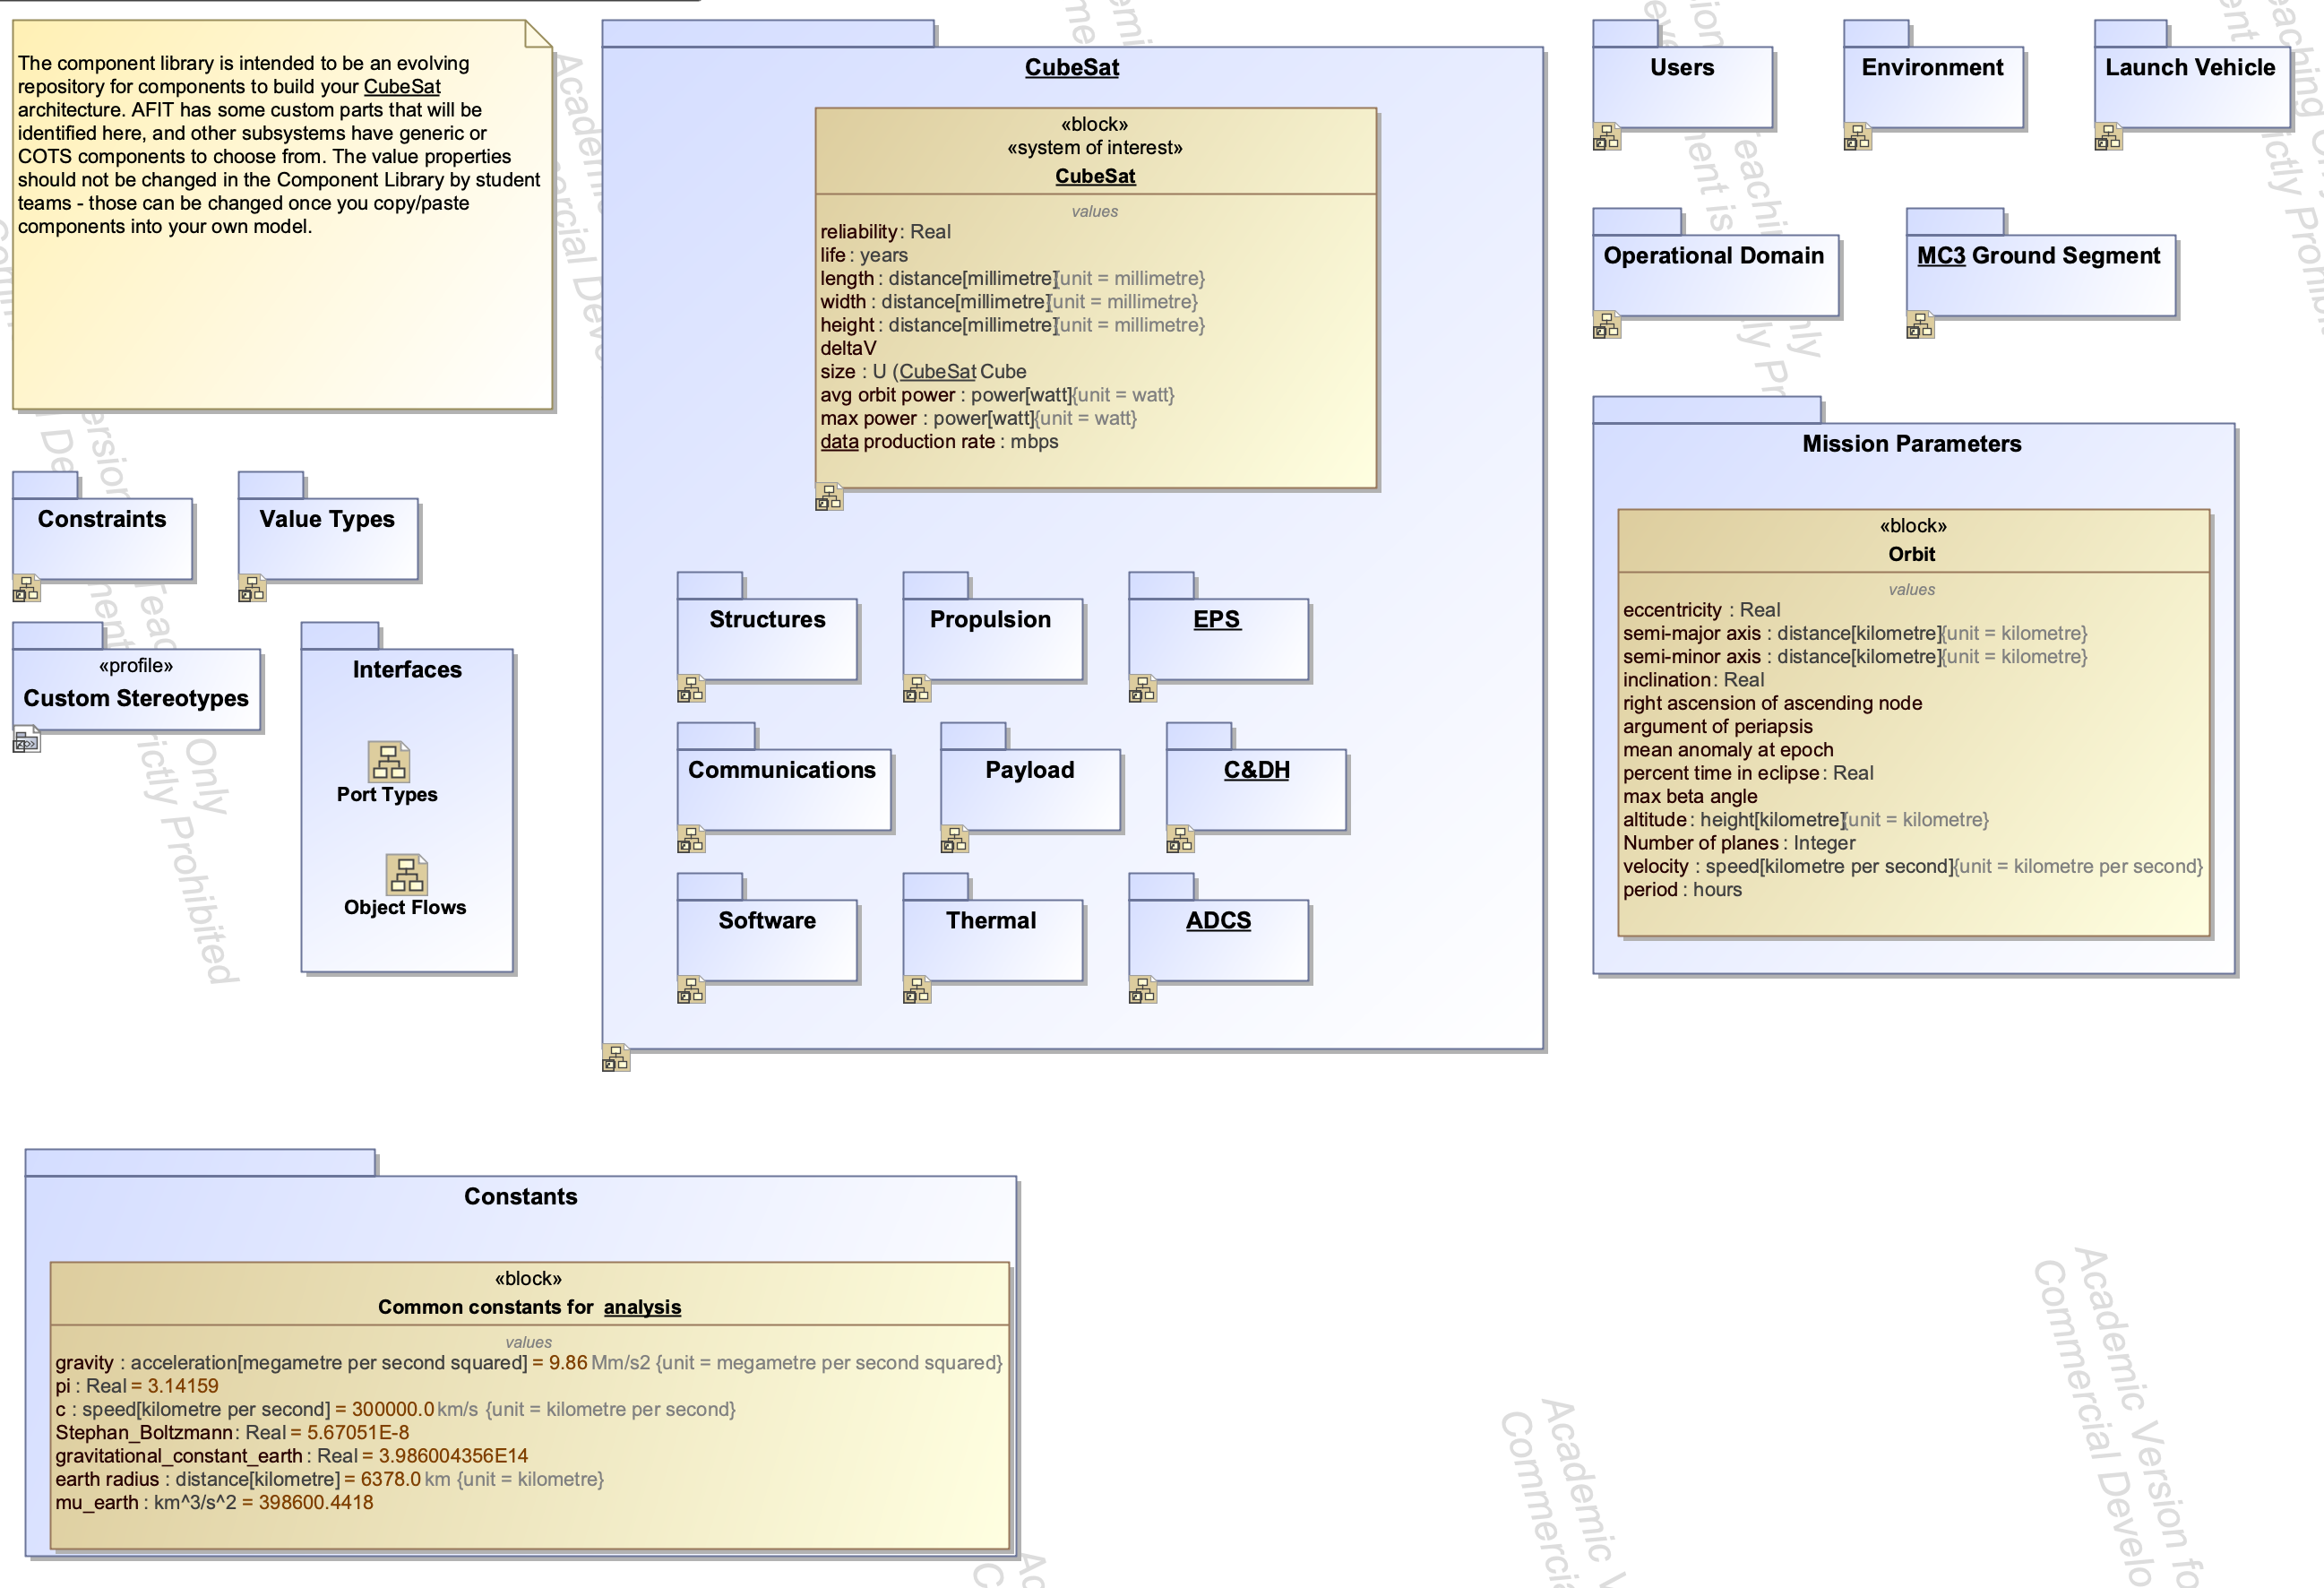
\includegraphics[width=\textwidth]{Figures/Component Library.png}
    \caption{Component Library Organization}
    \label{fig:Component Library Organization}
\end{figure}

The third package is the core of the Reference Architecture. The "Generic CubeSat Model" is the template that teams will start from. It has a pre-built, "mission-less" CubeSat model with diagrams, tables, and matrices provided with template data that is meant to be replaced by the design teams. It also contains the Document Generator tools that will be discussed later. Each package within the "Generic CubeSat Model" is hyperlinked to an informative splash page linking to all of the included tools and instructions for how to navigate them. Those splash pages are shown below in Figures \ref{fig:Requirements Organization} through \ref{fig:Document Generator Organization}.
\begin{figure}
    \centering
    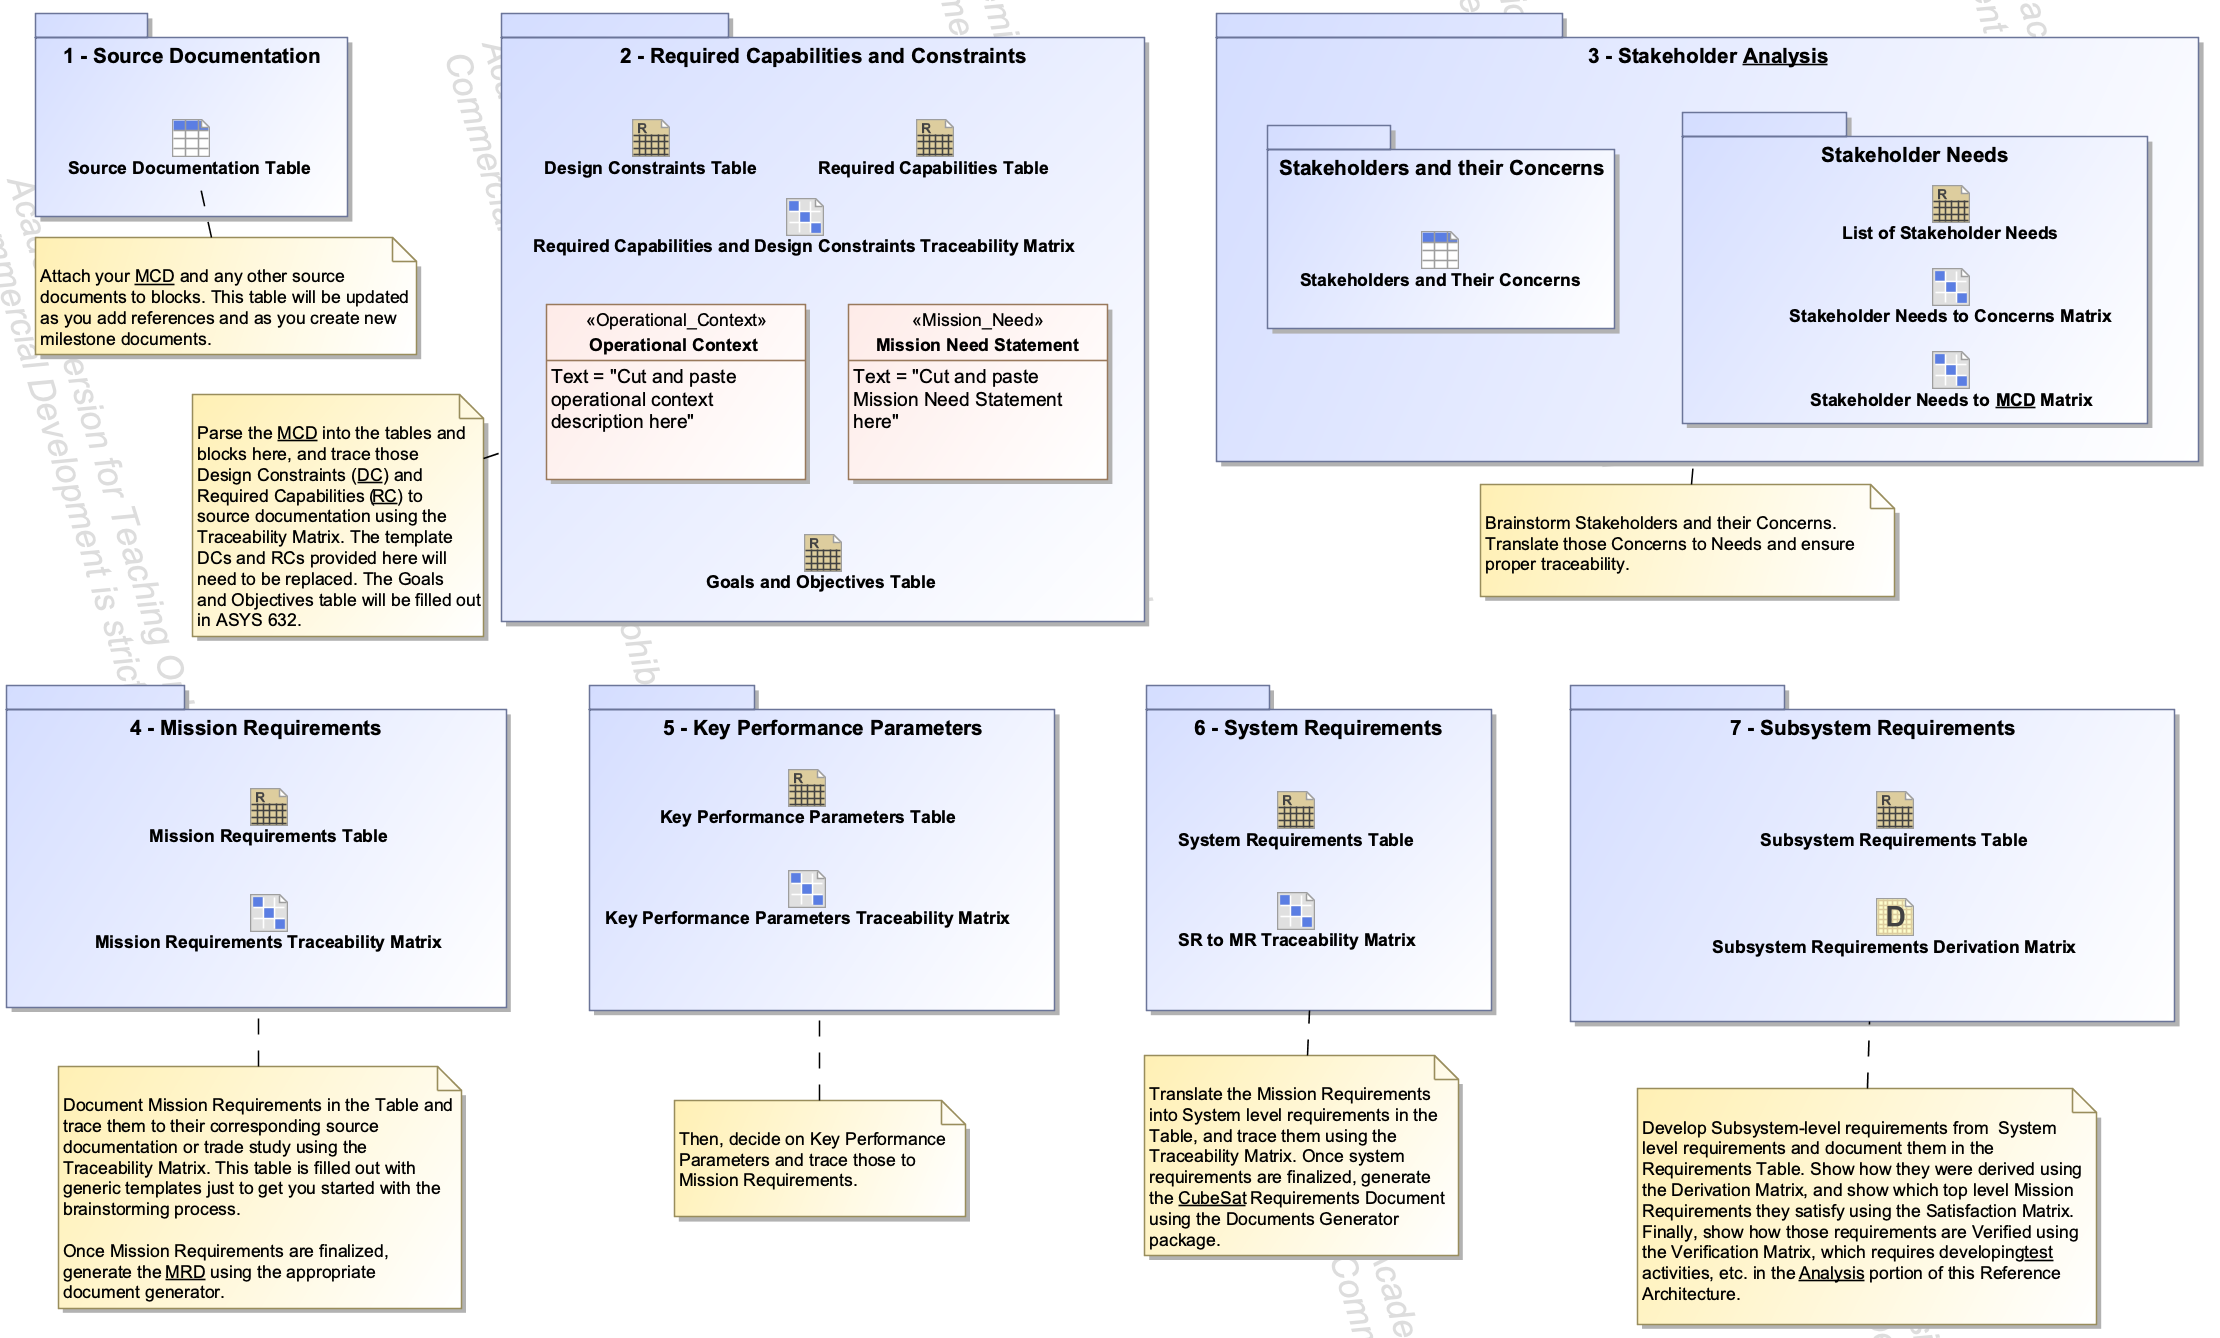
\includegraphics[width=\textwidth]{Figures/Requirements Organization.png}
    \caption{Requirements Organization}
    \label{fig:Requirements Organization}
\end{figure}

\begin{figure}
    \centering
    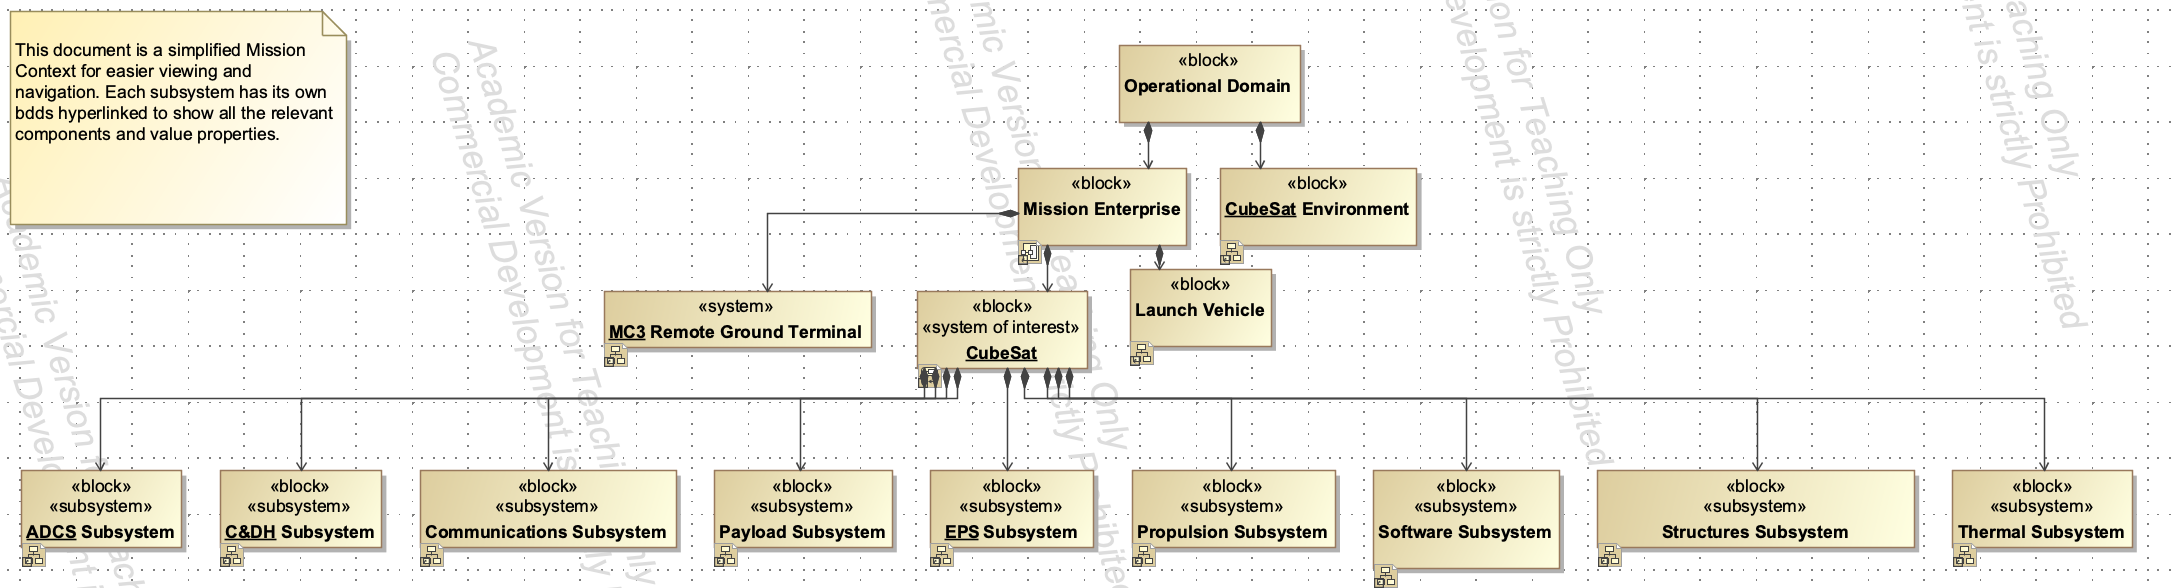
\includegraphics[width=\textwidth]{Figures/Physical Decomp.png}
    \caption{Structure Organization}
    \label{fig:Structure Organization}
\end{figure}

\begin{figure}
    \centering
    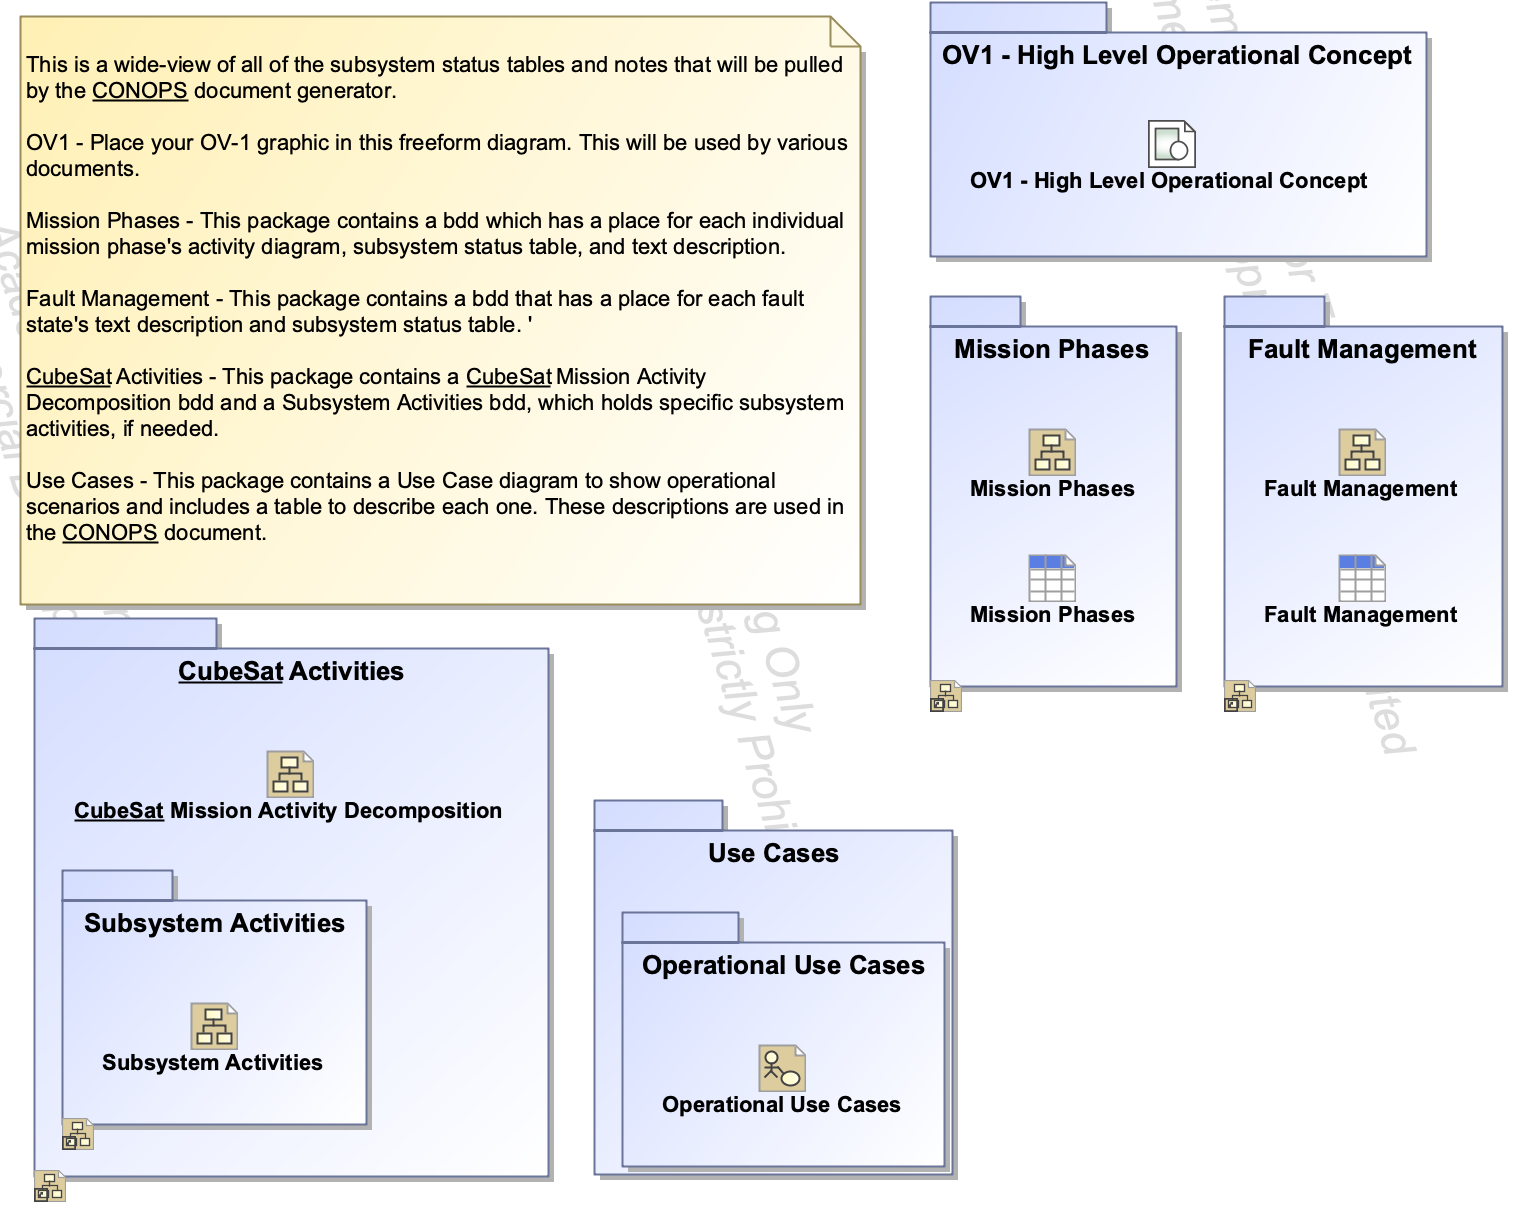
\includegraphics[width=\textwidth]{Figures/Behavior Organization.png}
    \caption{Behavior Organization}
    \label{fig:Behavior Organization}
\end{figure}

\begin{figure}
    \centering
    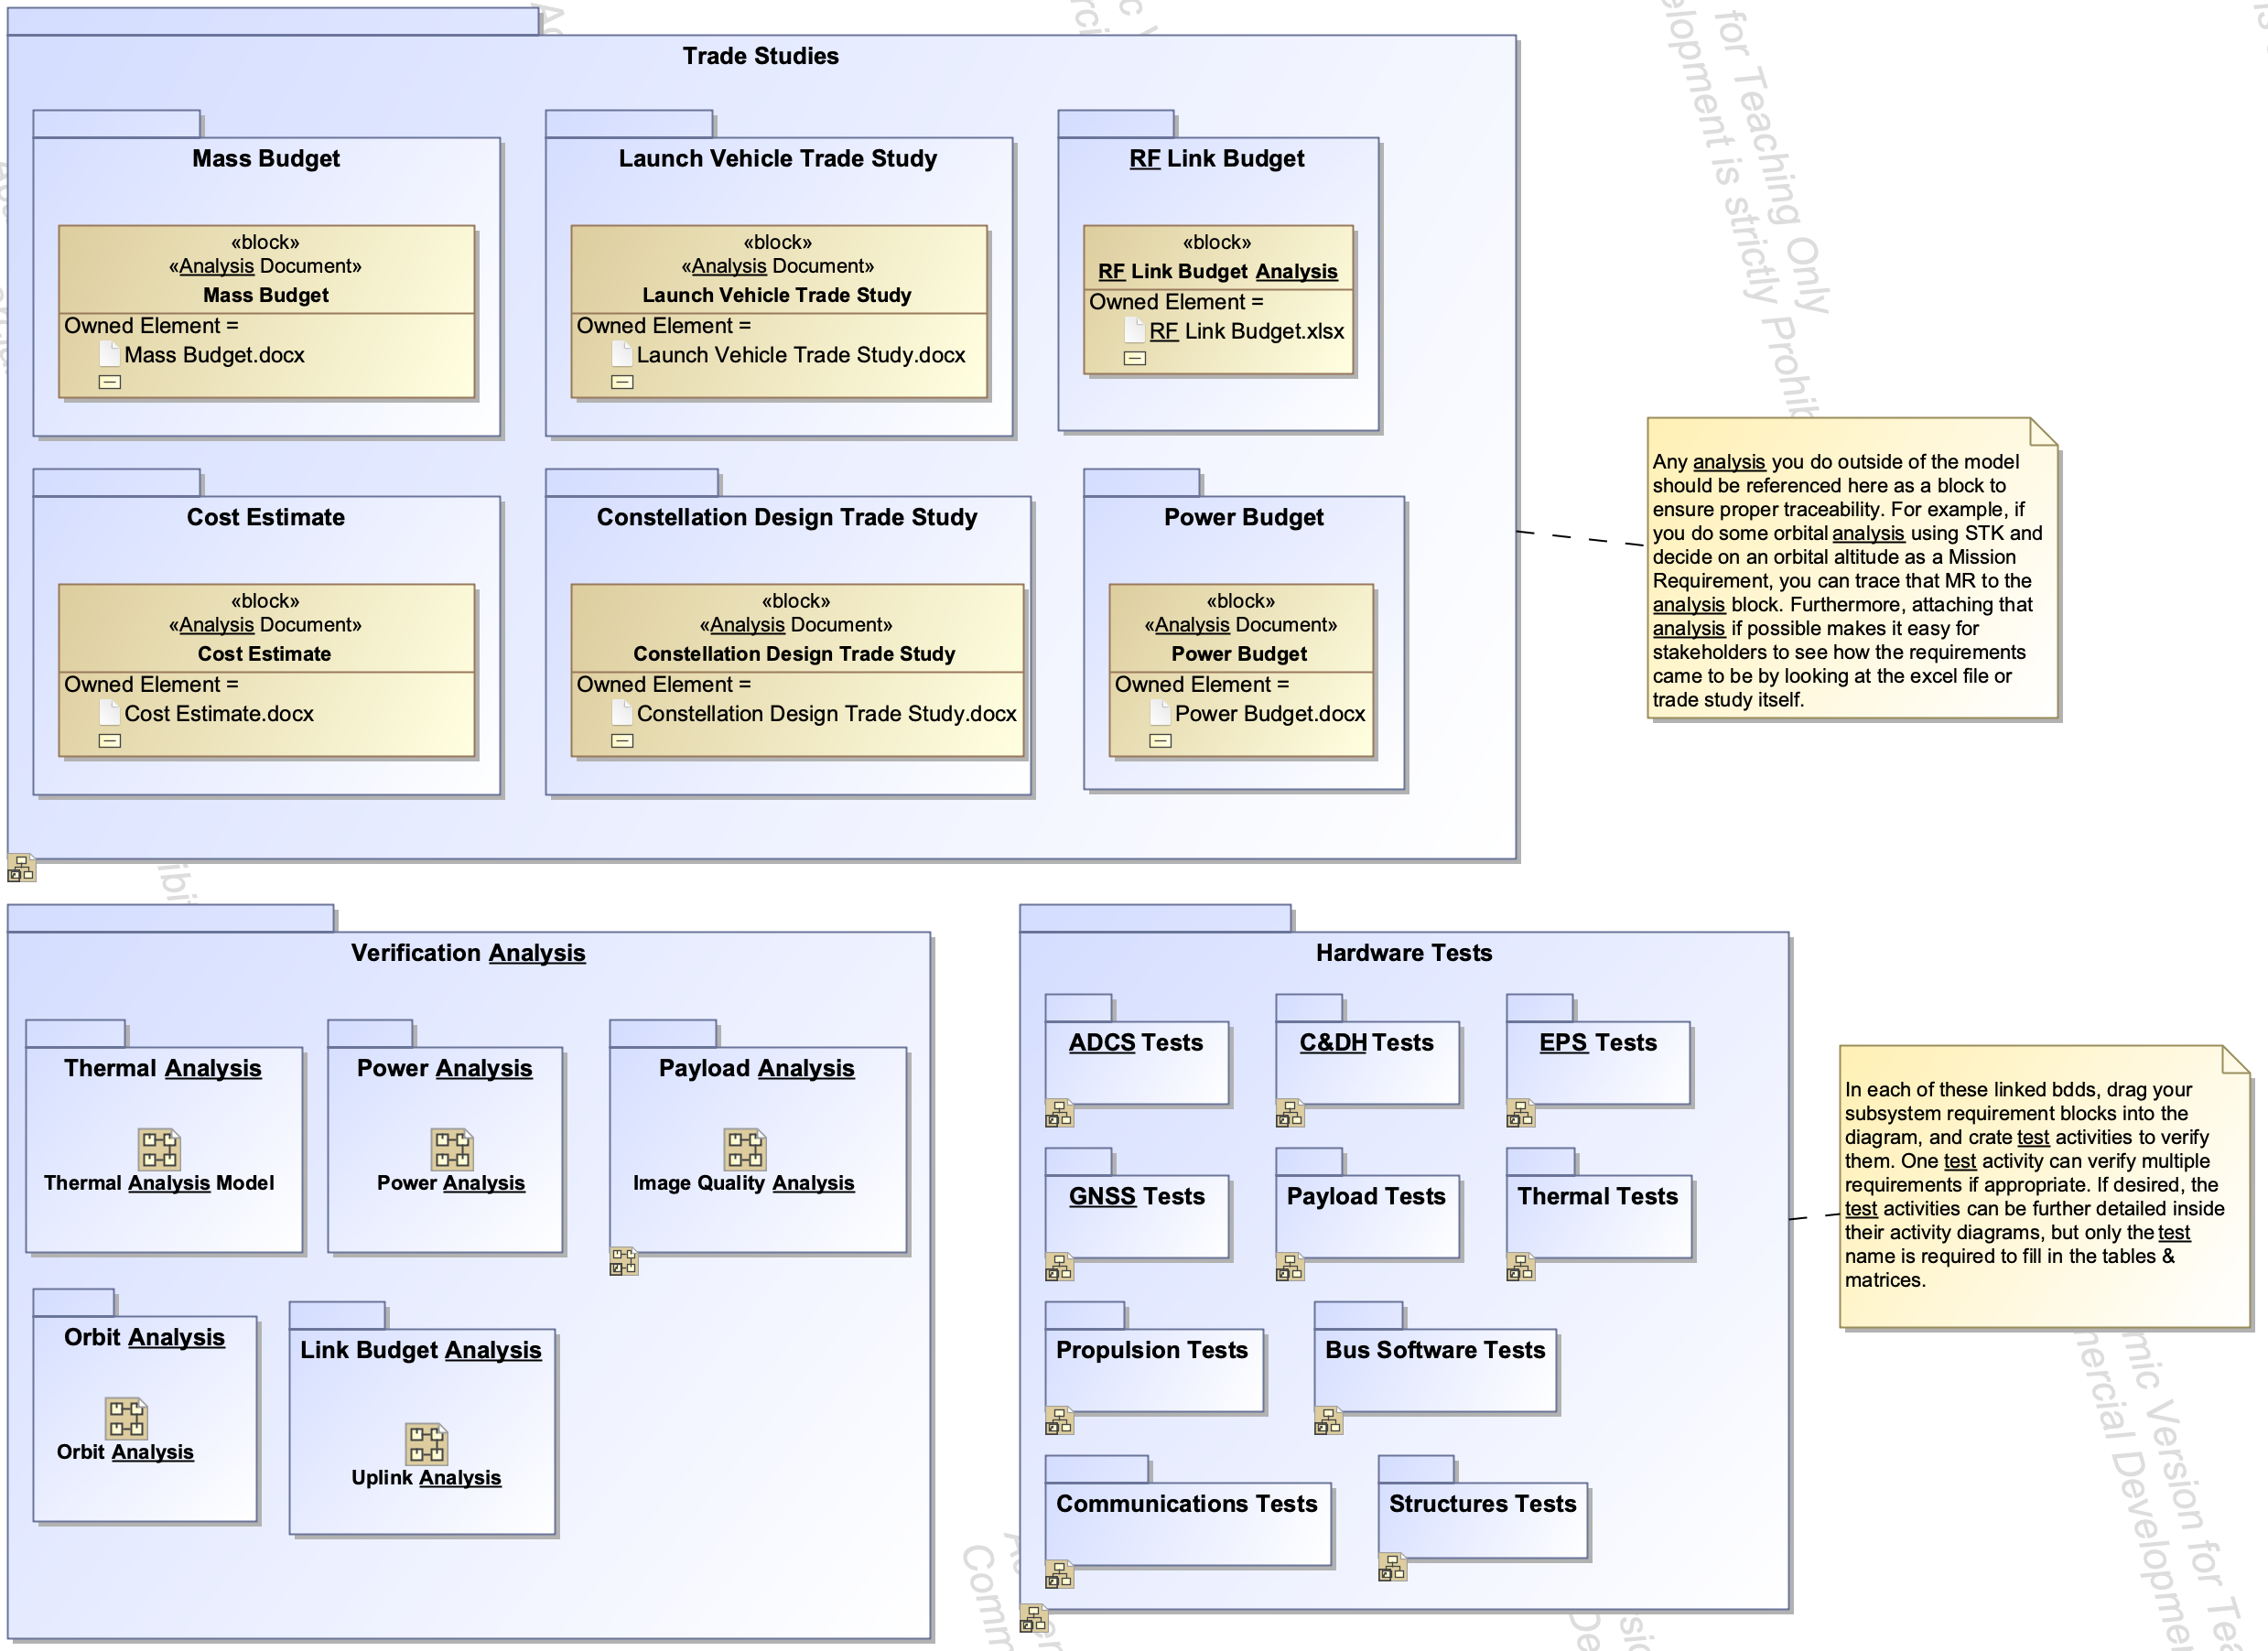
\includegraphics[width=\textwidth]{Figures/Analysis Organization.png}
    \caption{Analysis Organization}
    \label{fig:Analysis Organization}
\end{figure}

\begin{figure}
    \centering
    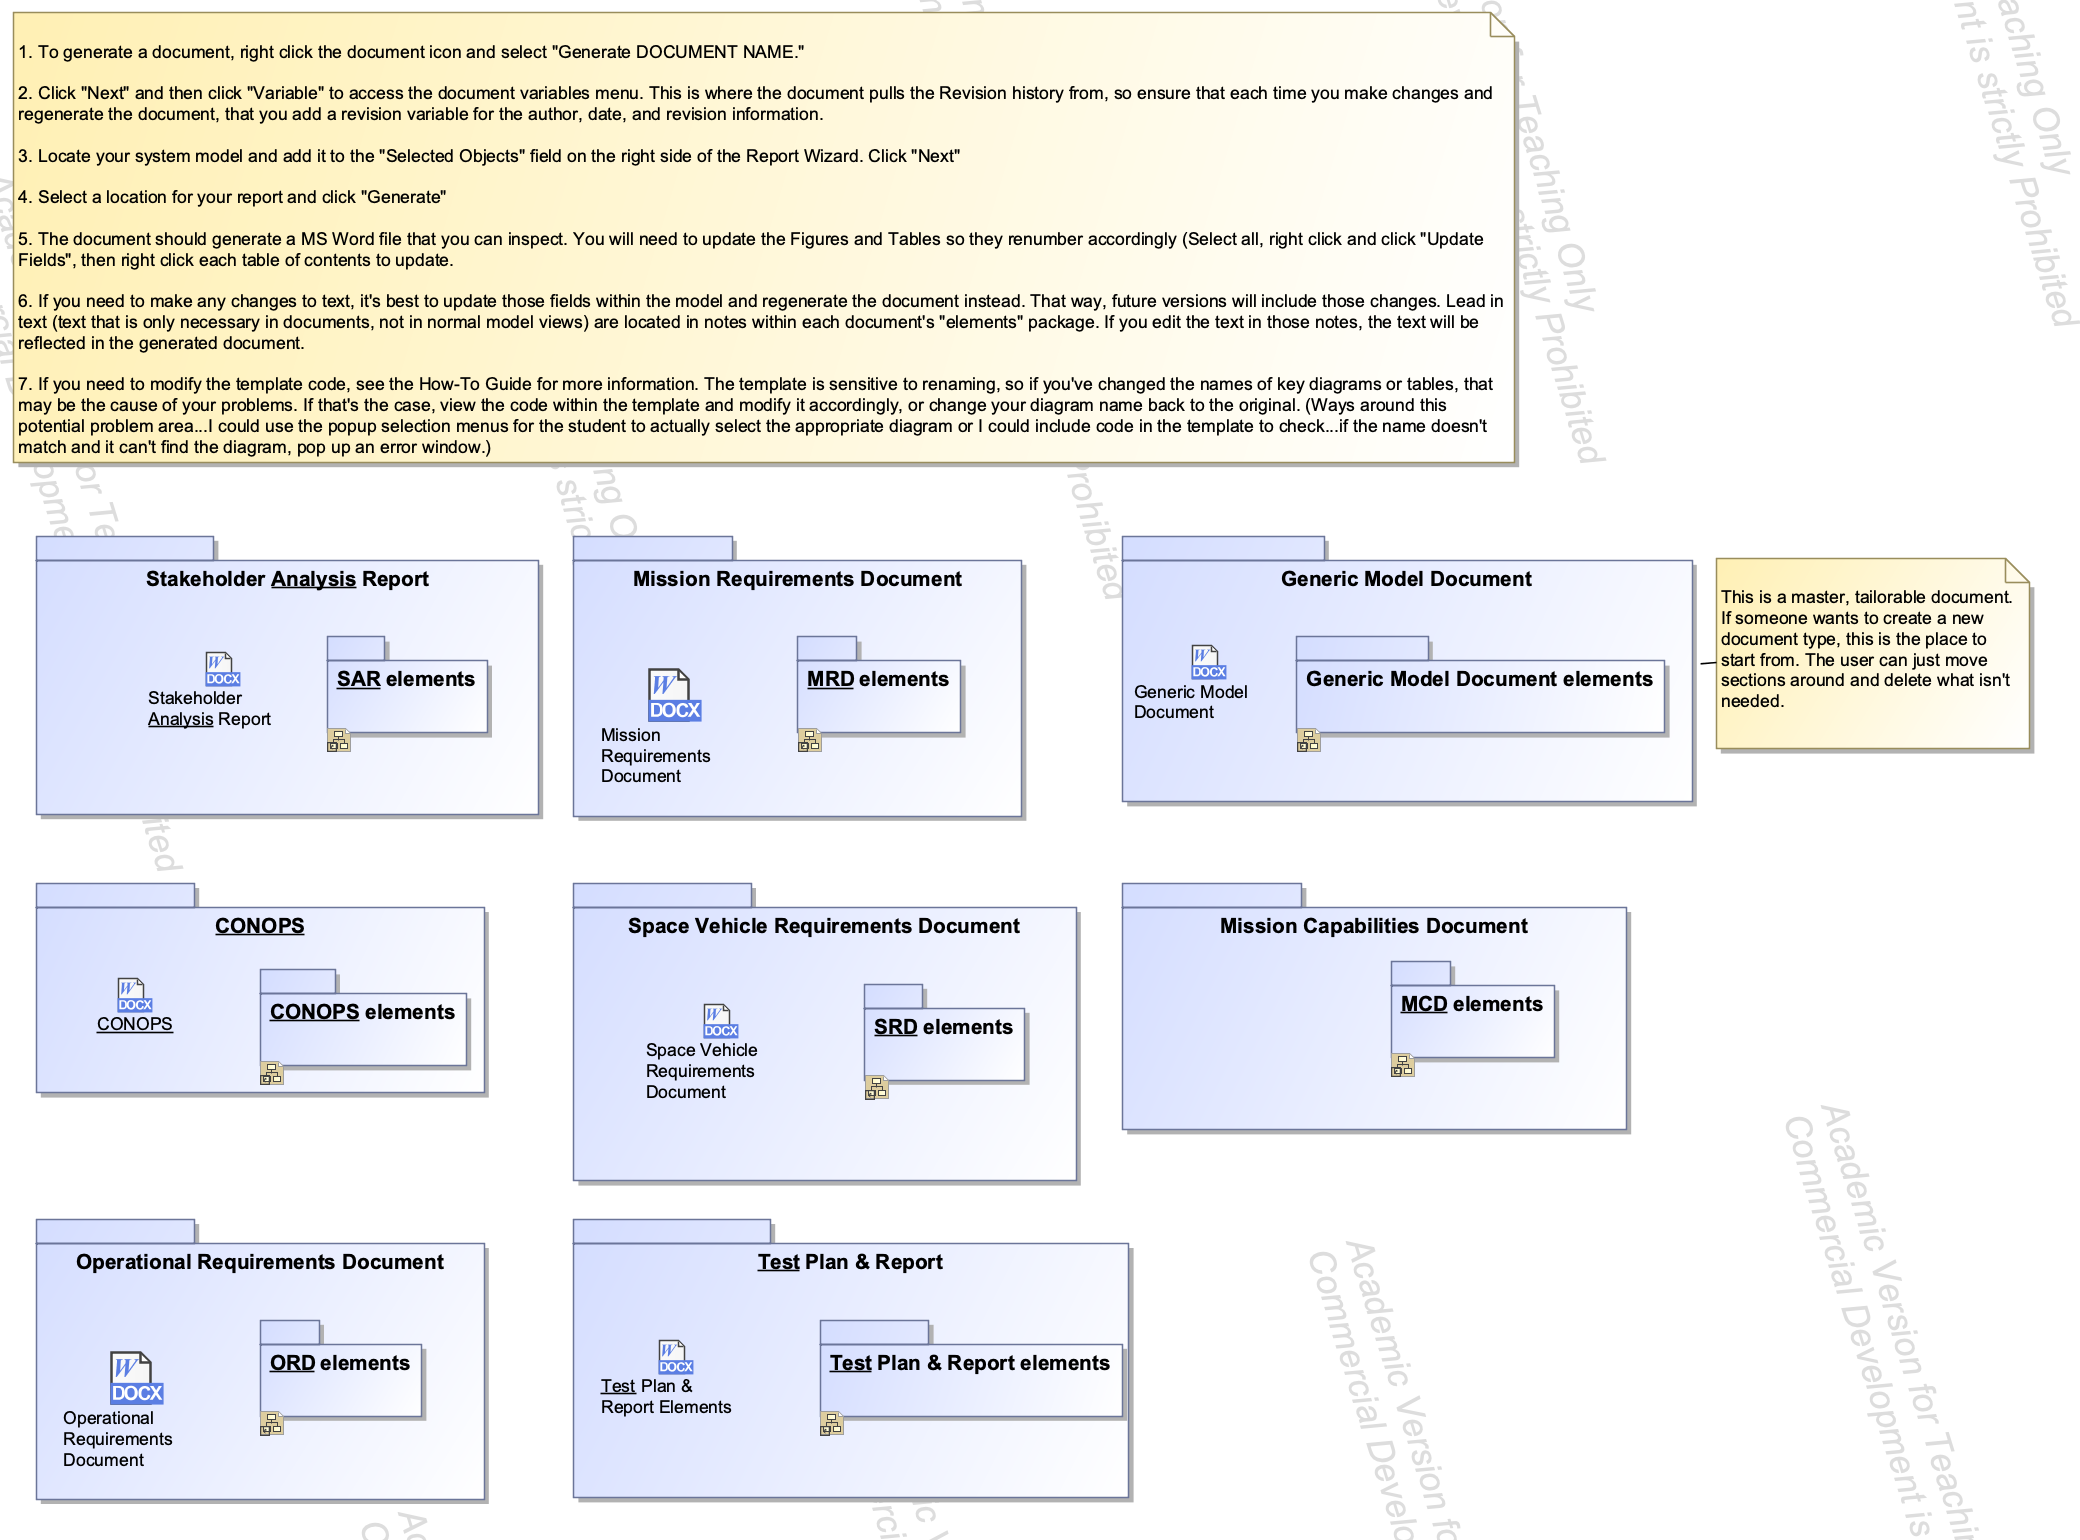
\includegraphics[width=\textwidth]{Figures/Document Generator Organization.png}
    \caption{Document Generator Organization}
    \label{fig:Document Generator Organization}
\end{figure}


The final package contains the various physical instantiations of the Reference Architecture. This could contain past projects to reference if needed, but for the purposes of the Reference Architecture development, it was used as the test-bed to validate the model. This is also where teams will place their starting template to build from, keeping the generic CubeSat model for future use. 


\subsection{Use of CubeSat Reference Architecture for Requirements Verification and Validation}
One of the key new functions of this CubeSat Reference Architecture is the Verification and Validation section. 

Figure \ref{fig:Analysis Organization} shows the Analysis portion of the Reference Architecture, which helps guide teams through the Requirement Verification and Validation processes. Because the CubeSat component blocks include predefined value properties, parametric diagrams could be created to perform a variety of calculations based off these values. Figure \ref{fig:Thermal Analysis} shows an example of a parametric diagram that can be used by the user to rapidly analyze their system. This Thermal Analysis parametric diagram includes a constraint block with MATLAB code. This MATLAB code uses value properties from the Thermal Subsystem block (radiating area, emissivity, absorbtivity, specific heat capacity, etc.), some parameters from the Orbit block (altitude, period, etc.), and any other value properties needed to perform the calculations. This MATLAB script outputs graphs, as shown in Figure \ref{fig:Thermal Analysis Results}, which change automatically if the user swaps out a new thermal subsystem block, changes the altitude, or otherwise modifies the value properties. For other analysis needs, the constraint blocks can output values instead of graphs, and these outputs can then be imported as value properties. 

\begin{figure}
    \centering
    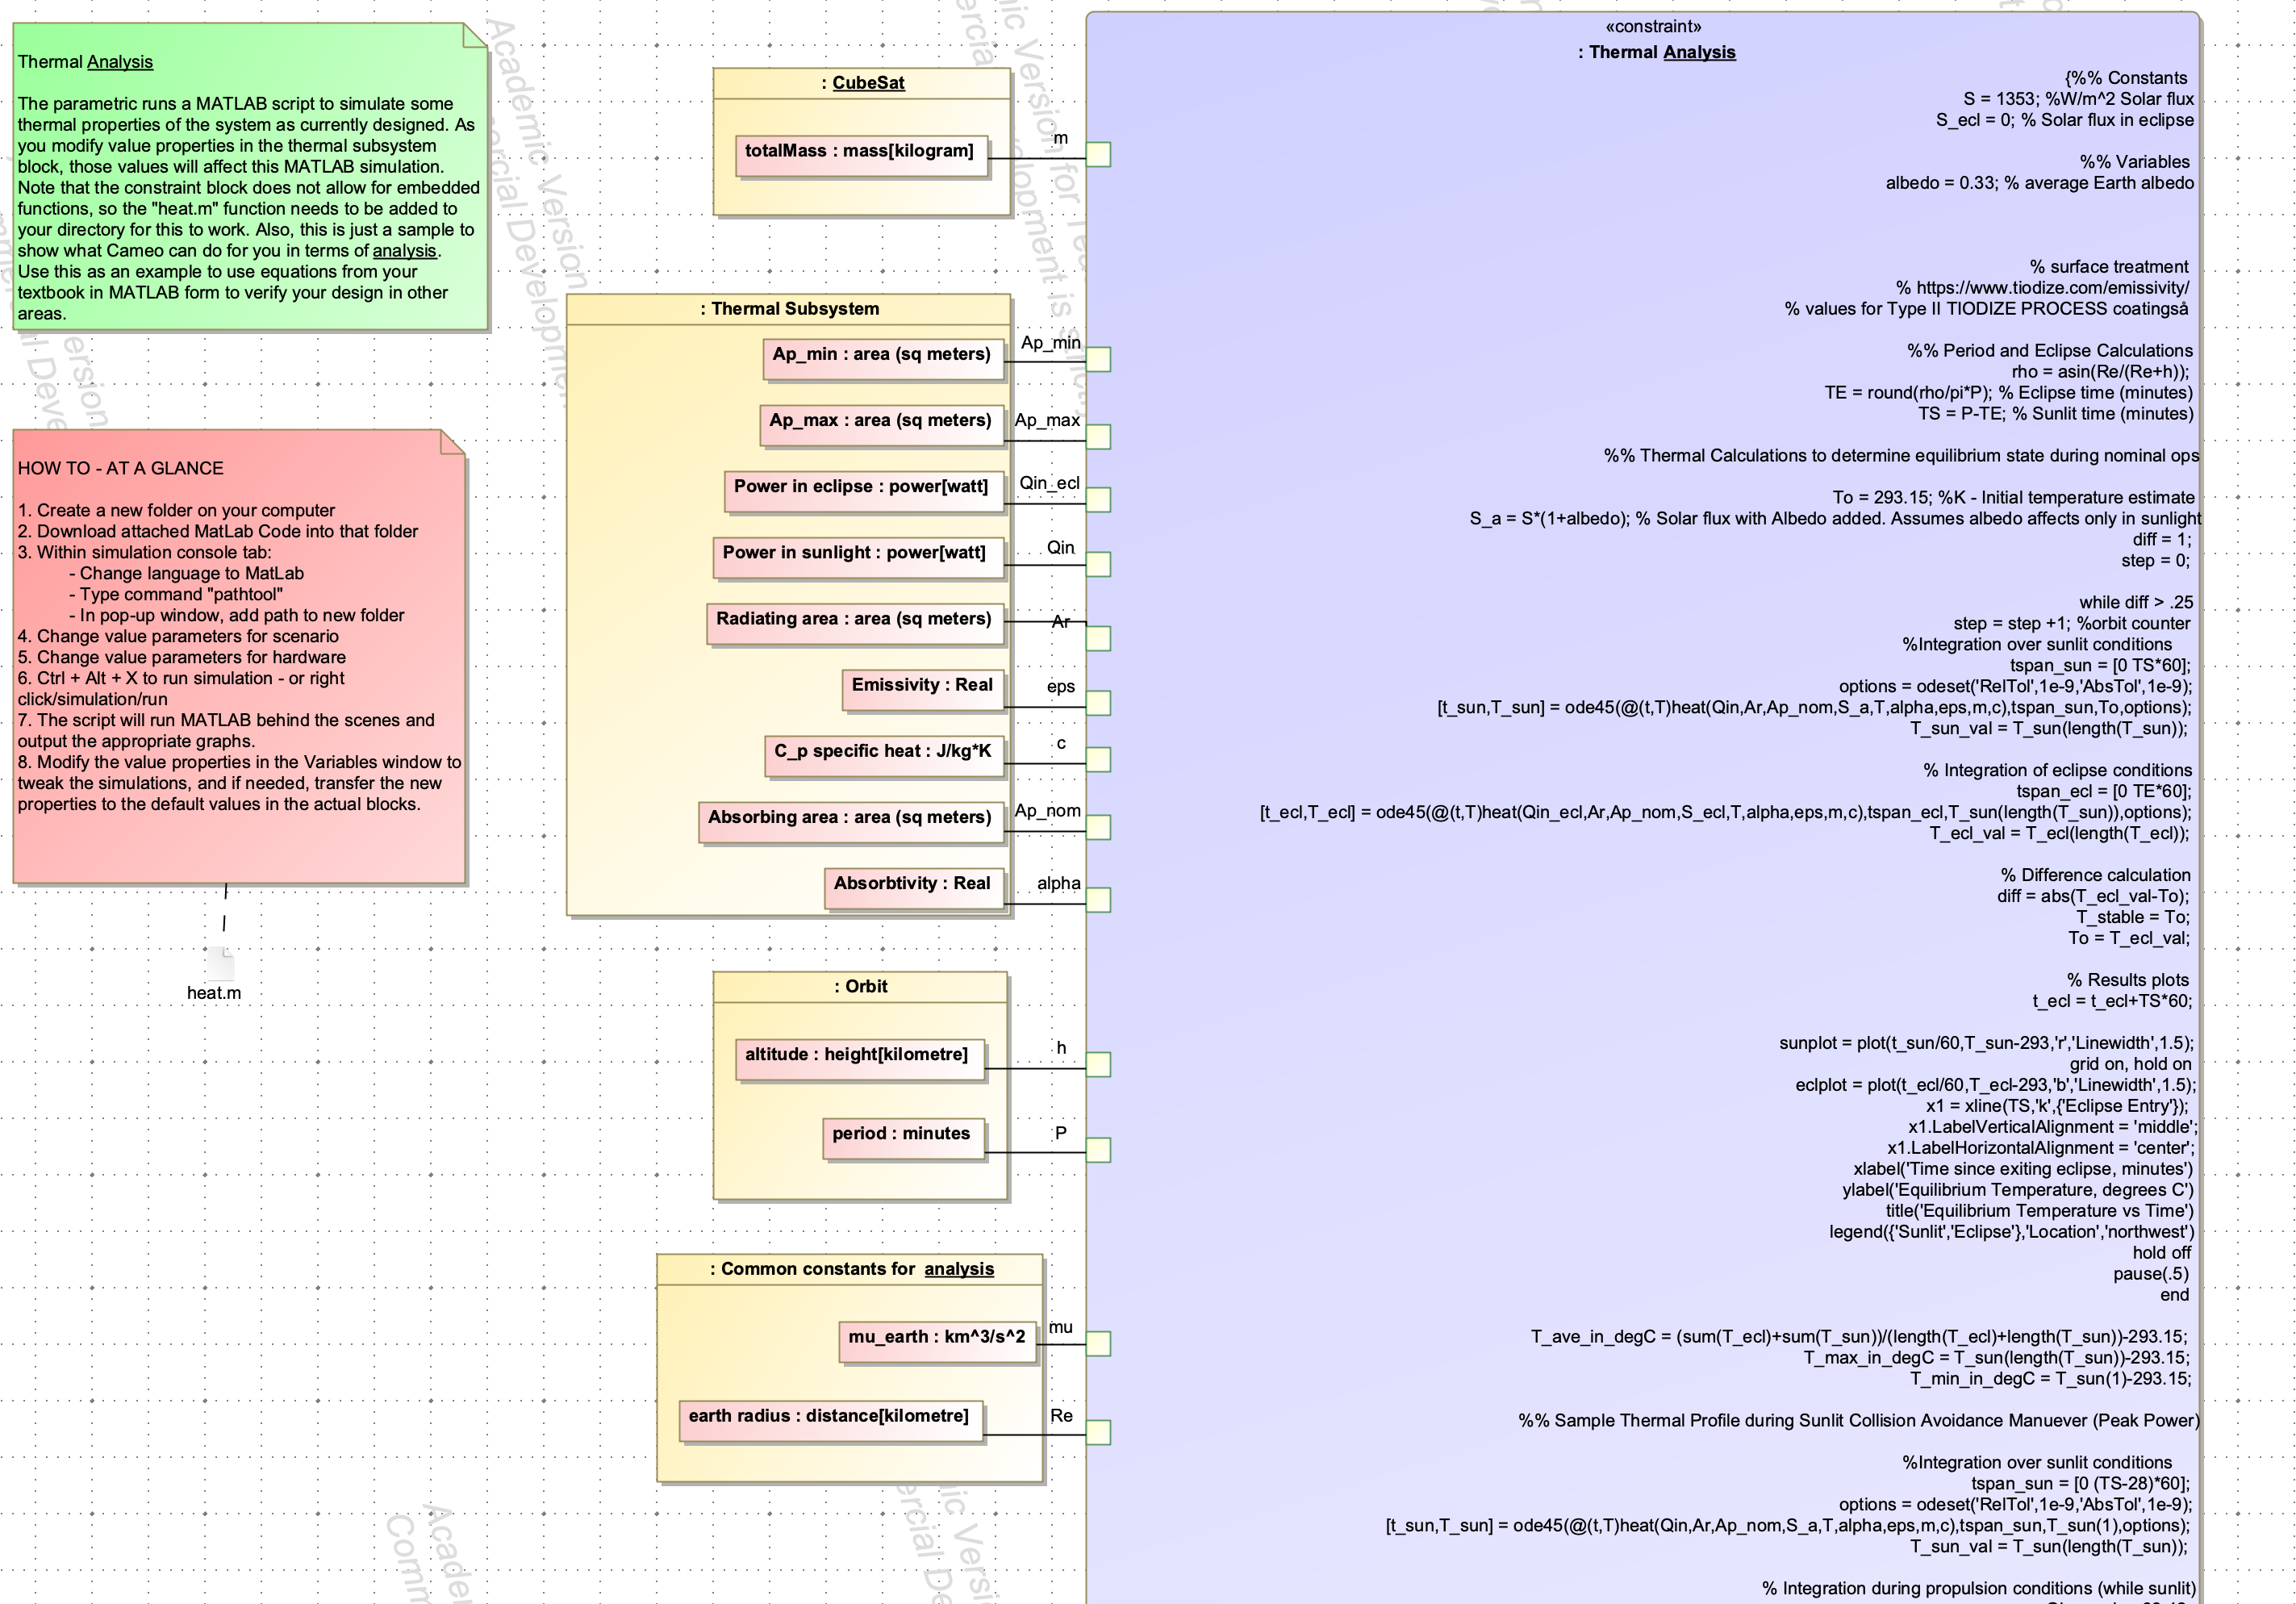
\includegraphics[width=\textwidth]{Figures/Thermal Analysis.png}
    \caption{Thermal Analysis}
    \label{fig:Thermal Analysis}
\end{figure}

\begin{figure}
    \centering
    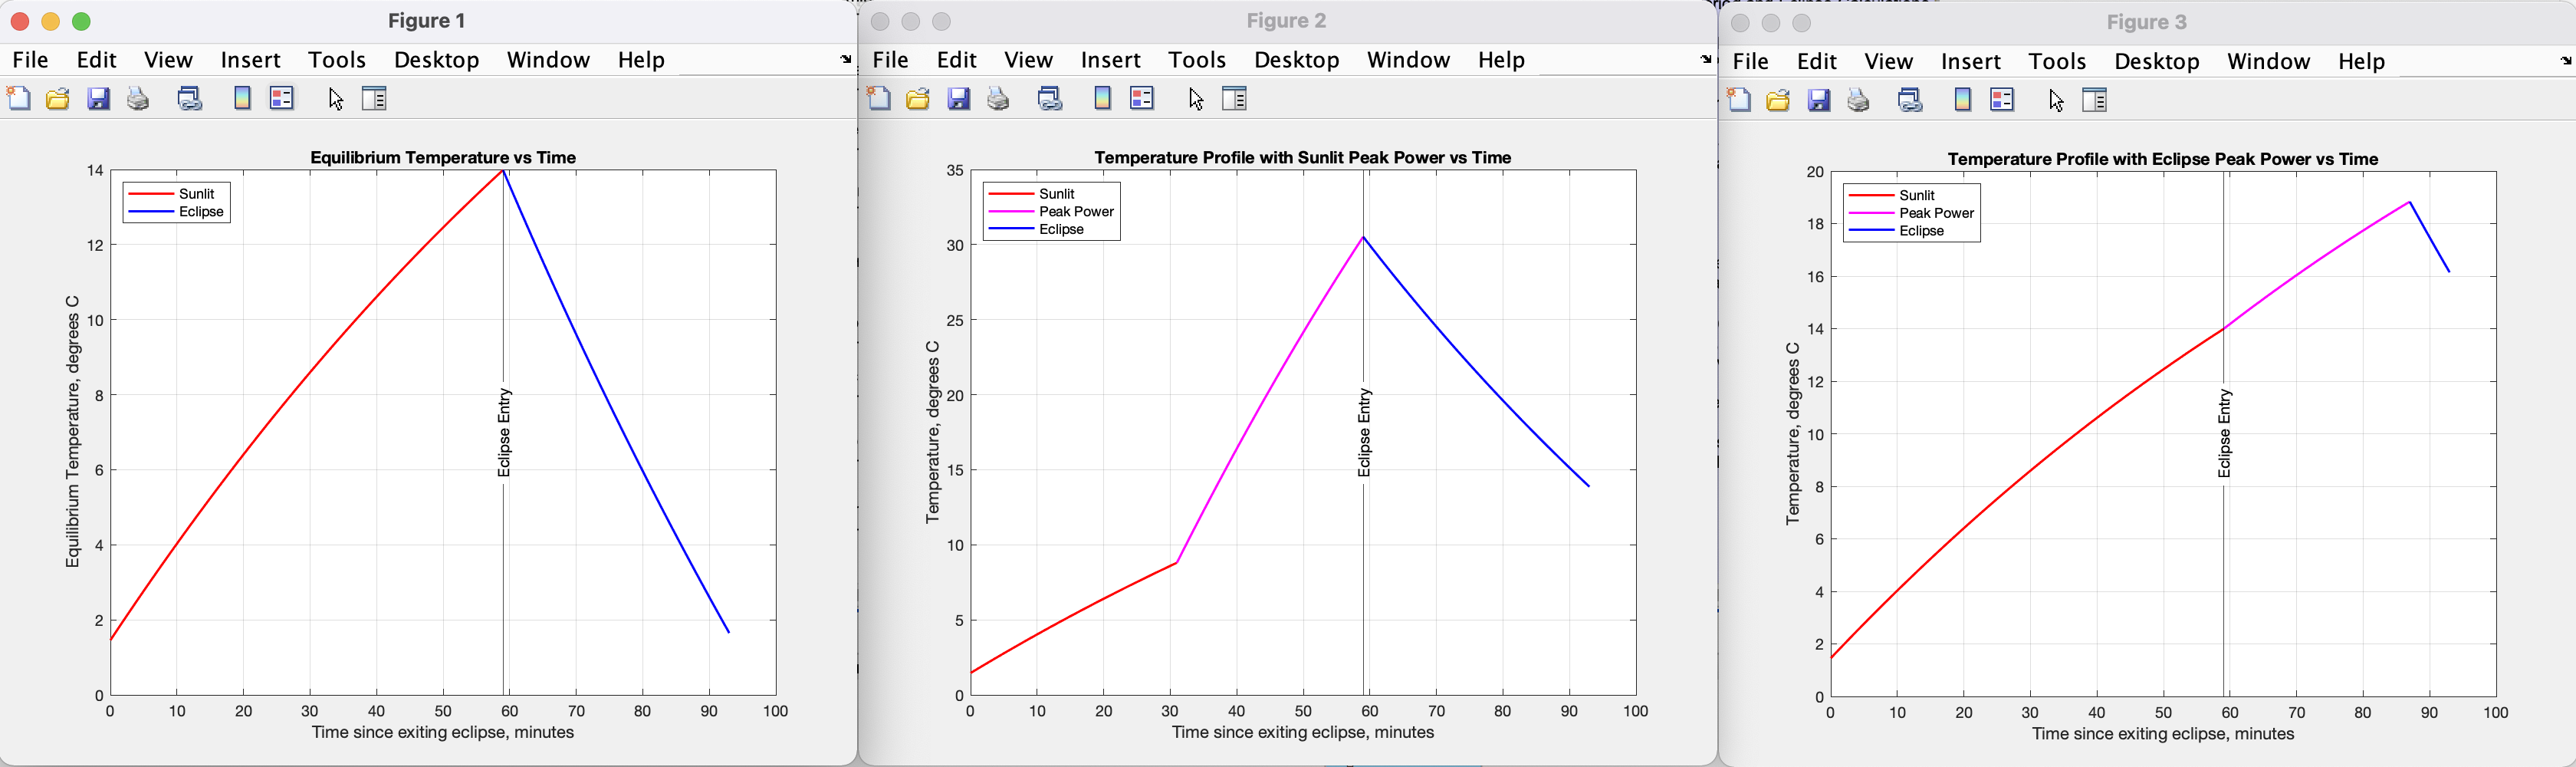
\includegraphics[width=\textwidth]{Figures/Thermal Graphs.png}
    \caption{Thermal Analysis Results}
    \label{fig:Thermal Analysis Results}
\end{figure}

The objective for the Analysis section of the Reference Architecture is to keep as much analysis contained within the model as possible, using the actual value properties to perform the calculations. Instead of taking values to other tools, the analysis calculations are kept within the model. Additional functionality can be added as well, depending on the requirements. For example, Figure \ref{fig:Image Quality Parametric Diagram} shows how a requirement for a "Near Infrared (NIR) Ground Sample Distance (GSD) of less than 4 m" could be tested using the same methodology. In this parametric diagram, the NIR GSD is calculated based off the imager's value properties and the CubeSat's altitude. This result is compared to the requirement and will automatically flag the result as green or red, depending on if it meets the requirement's constraint block or not, as shown in Figure \ref{fig:Image Quality Results}. 

\begin{figure}
    \centering
    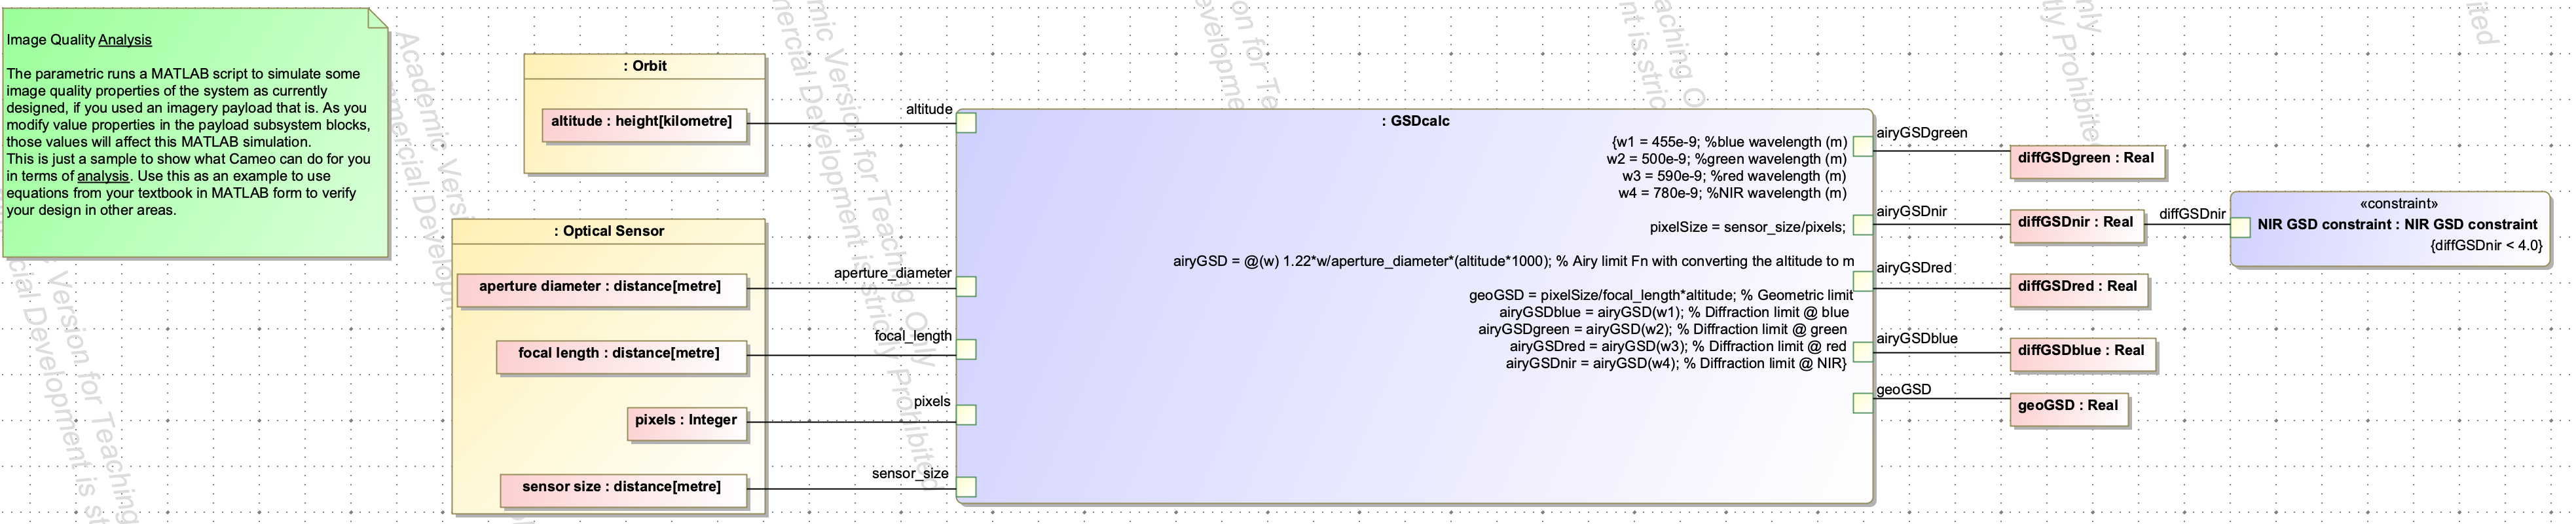
\includegraphics[width=\textwidth]{Figures/image quality.png}
    \caption{Image Quality Parametric Diagram}
    \label{fig:Image Quality Parametric Diagram}
\end{figure}

\begin{figure}
    \centering
    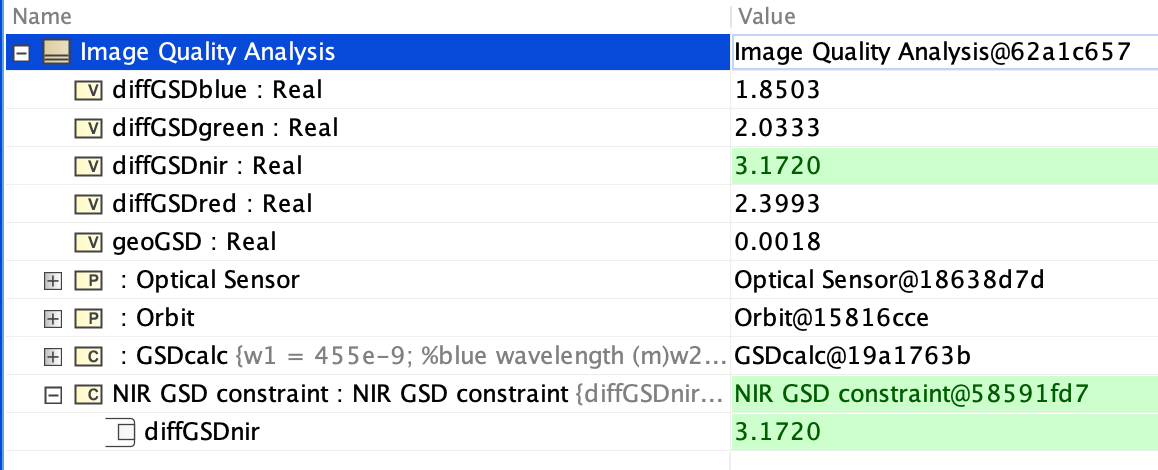
\includegraphics[width=\textwidth]{Figures/image quality results.png}
    \caption{Image Quality Results}
    \label{fig:Image Quality Results}
\end{figure}

With the included examples, teams can see the format and process to integrate outside tools such as MATLAB and AGI's Systems Toolkit (STK) to perform quick analysis based off model data. 

In addition to the parametric diagrams, teams will need to perform hardware tests in the lab, and the Reference Architecture accounts for that as well. There is a package for the hardware tests for each subsystem with features to help keep everything organized. Figure \ref{fig:ADCS Tests} shows the testing diagram for the Attitude Determination and Control Subsystem (ADCS). The user can access the applicable requirements in the linked subsystem requirement table, create test activities to verify requirements, and include descriptions of each test in the included test description table. The linked subsystem requirement tables are automatically generated and also include color coding to highlight testing status. As tests are completed, the user can choose a verification status from a dropdown menu (such as Requirement Verified, Test Not Completed, Testing in Progress, etc.), as shown in Figure \ref{fig:ADCS Requirement Table}. 

\begin{figure}
    \centering
    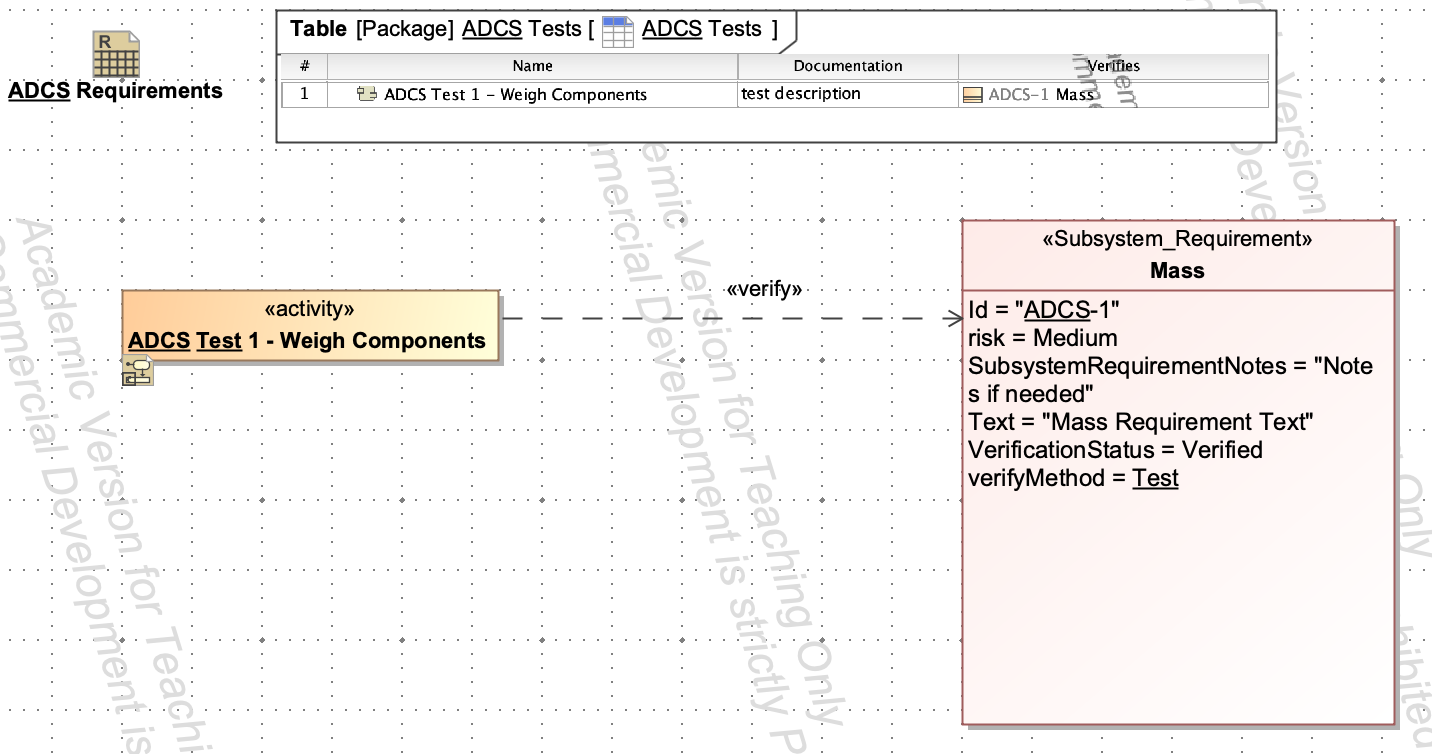
\includegraphics[width=\textwidth]{Figures/ADCS tests.png}
    \caption{ADCS Tests}
    \label{fig:ADCS Tests}
\end{figure}

\begin{figure}
    \centering
    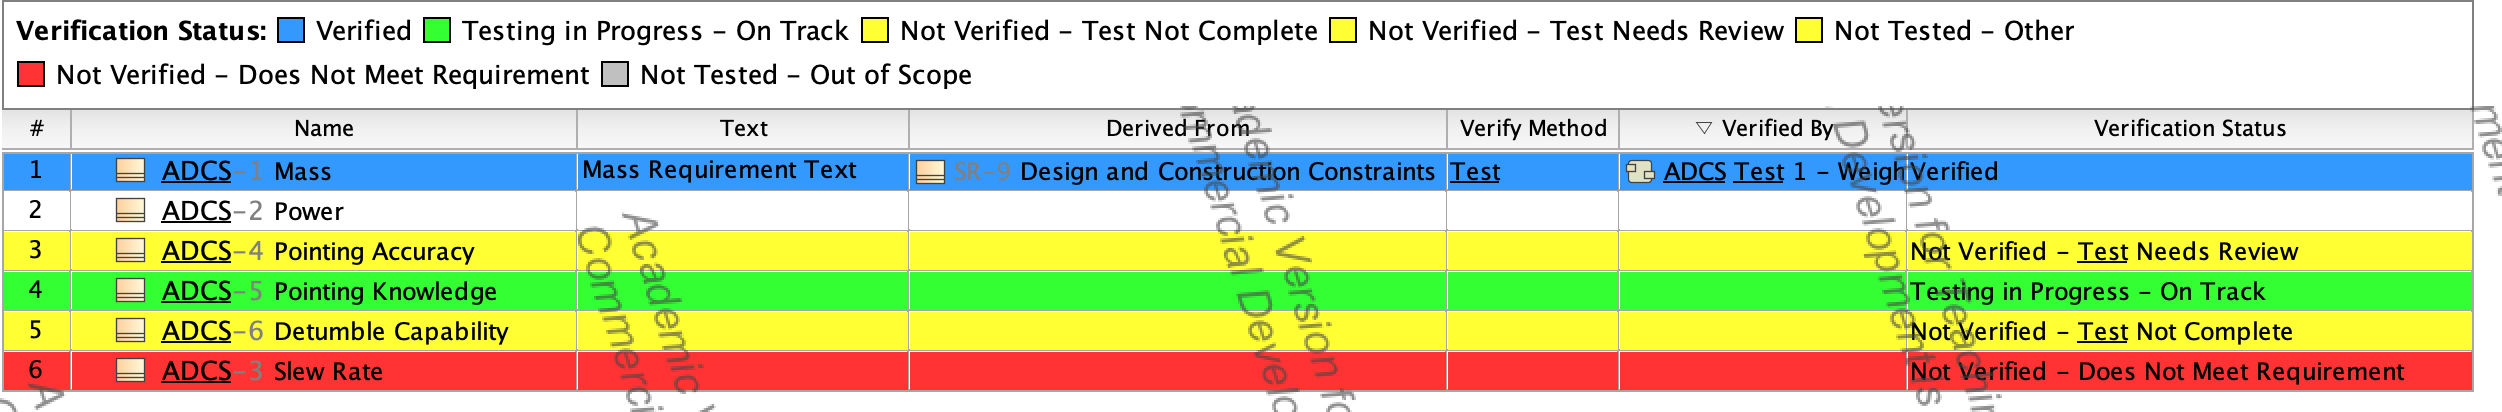
\includegraphics[width=\textwidth]{Figures/ADCS requirement table.png}
    \caption{ADCS Requirement Table}
    \label{fig:ADCS Requirement Table}
\end{figure}

\subsection{Use of CubeSat Reference Architecture for Generating Traditional Documentation}
This Reference Architecture includes polished document generator functionality. Cameo Systems Modeler can use Apache's Velocity Template Language (VTL) to export model elements into external tools such as Microsoft Word and Microsoft PowerPoint. By including Microsoft Word file templates with tailored VTL code, documents can be automatically generated as needed as the model is updated. Even narrative text, such as introduction paragraphs or other lead-in text, can be included within the model as Notes. The Reference Architectures includes document generators for a Stakeholder Analysis Report (SAR), Concept of Operations (CONOPS), Mission Requirements Document (MRD), Operational Requirements Document (ORD), Space Vehicle Requirements Document (SRD), Mission Capabilities Document (MCD), and a document to help start Test Plans. The templates were based off of AFIT course requirements, but they may be tailored if different sections are required or if the order of sections needs to be modified. Additionally, the Reference Architecture includes a template for a master generic model document, which just exports all model elements that the team generated in an intuitive and visual format. This is useful as it contains all code that a user may wish to use if they want to create a new document template that was not provided. The generic model document can be used as a template to build custom documents from. The first page of the generic document template is shown below to show what the code looks like. The generic template is commented so users can know how it works and what to copy for a new document. Figure \ref{fig:VTL Example} shows the first page of the generic document template to show the general structure.

\begin{figure}
    \centering
    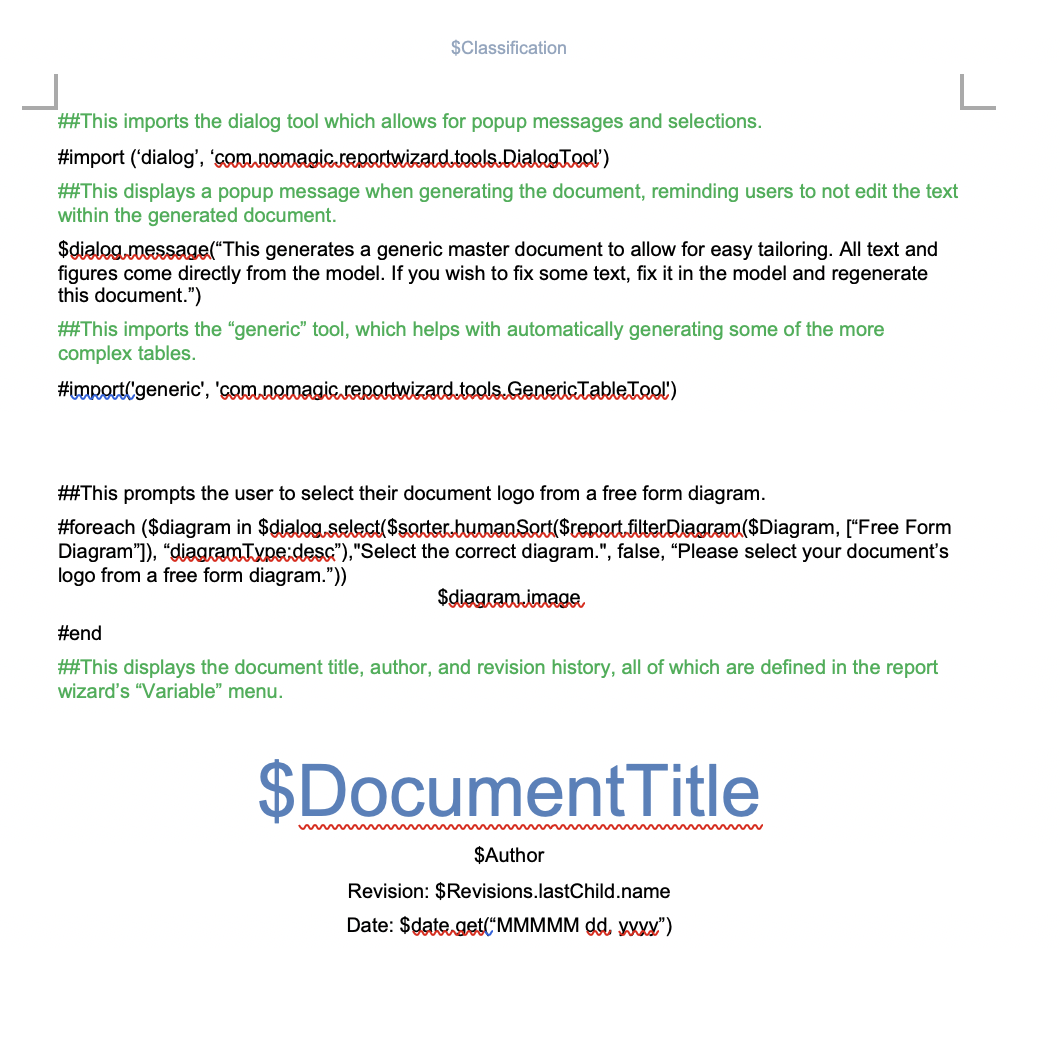
\includegraphics[width=\textwidth]{Figures/VTL example.png}
    \caption{VTL Example}
    \label{fig:VTL Example}
\end{figure}

The goal of these document generators is to encourage the use of the model throughout the sequence. Traditionally, teams would have to copy and paste model elements into reports and transcribe requirement text into MS Word or PowerPoint tables for reviews or deliverables. This led to version control issues, such as requirement text being updated in the PowerPoint table but not in the underlying model. By keeping everything entirely within the model, these document generators take much of the manual work out of the process. Teams can focus on ensuring the model is accurate instead of needing to cross-check every diagram each time a change is made.

The document generators feature multiple ways to import data. For example, when importing a table, the table columns can be specifically called out using VTL, or the table can be generated as it appears in the model. Each method has benefits, so both were included in the master template. Figure \ref{fig:VTL Table Methods} shows both table methods for displaying the "System Requirements Table" as an example. The first method allows the user to choose which columns are imported and in what order they appear, while the second method just imports the table exactly as it appears in the current model. Some tables are very large, so the first method may be preferable if only a few columns are required. The code syntax instructions are provided within the template if different model data needs to be imported. 

The primary downside to this tool is that many diagrams are called out by name in the template code. The names are generic names that don't need to be changed, but if teams wish to change the names of key tables or diagrams, the template will not import the applicable data. This is easily remedied with a quick change to the template code to match the new diagram name, but this may cause some confusion if the generated documents don't contain everything the user thought it would. Anywhere a diagram is called out by name in the template code, that name is highlighted so it will be easy to locate and modify if ever needed. 

\begin{figure}
    \centering
    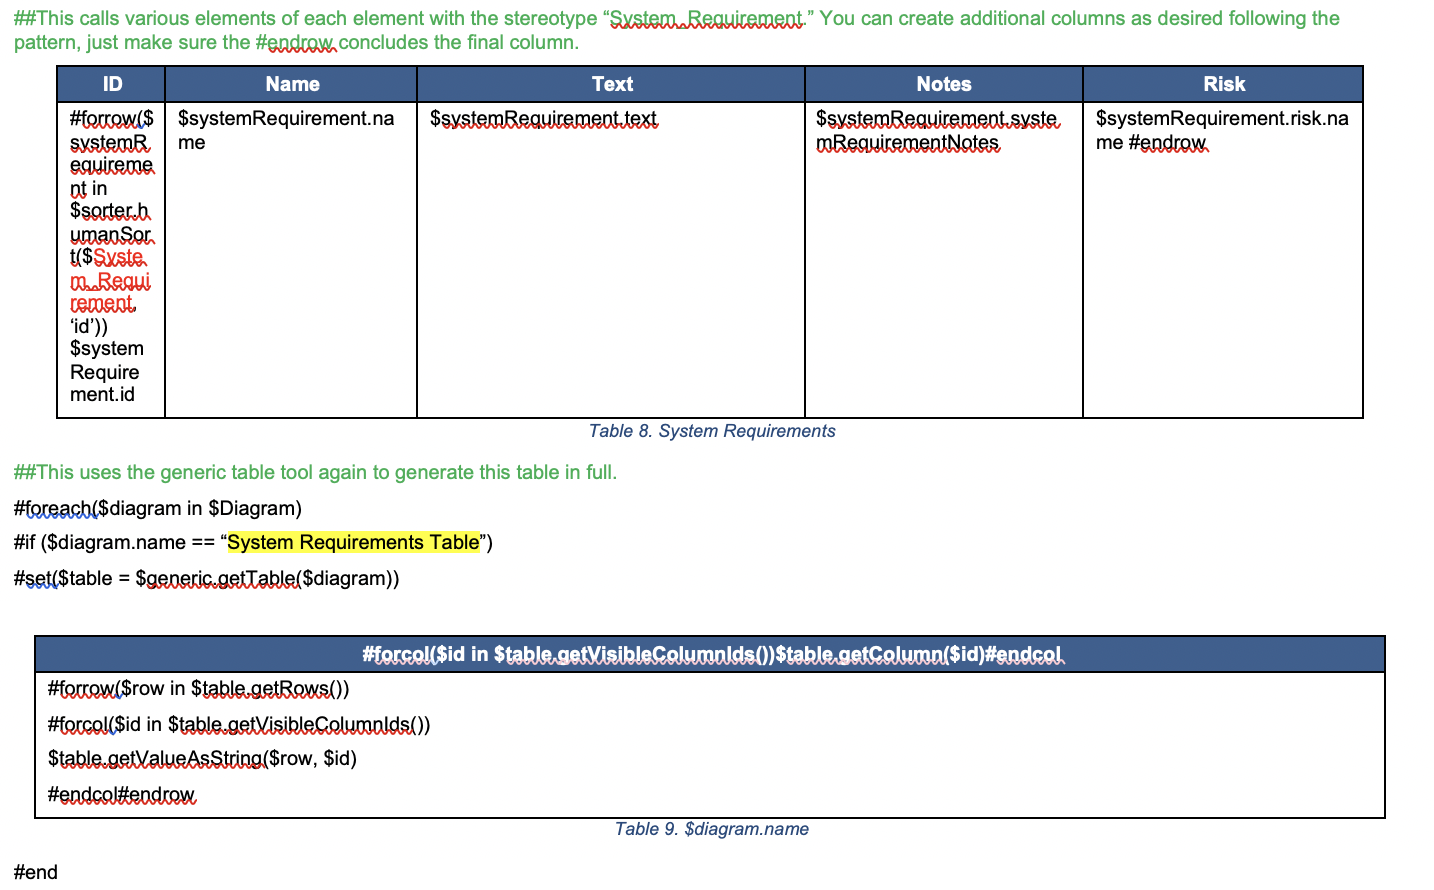
\includegraphics[width=\textwidth]{Figures/two kinds of tables.png}
    \caption{VTL Table Methods}
    \label{fig:VTL Table Methods}
\end{figure}

\section{Future work}
To date, the CubeSat Reference Architecture effort has been to establish a working template to test with the next batch of Space Systems Engineering students at AFIT. As the course sequence curriculum changes and as more people look at and use this Reference Architecture, improvements can and should be made for the benefit of future teams. The Reference Architecture as-is has been tested by prior students, but every team has different styles and preferences, and the Reference Architecture can reflect those differences.

As far as planned improvements go, the Component Library has just been started and will improve as the Reference Architecture is used by design teams. After design teams add components to their physical configurations, those components can be added to their respective subsystem package within the Component Library. After several iterations, there will be several different kinds of payloads to choose from, multiple propulsion systems, chassis sizes, etc. The Component Library can also hold other non-physical blocks for reuse as well, such as constraint blocks for analysis, object flows, value types, and custom stereotypes.

Furthermore, the Analysis section includes several working examples that work with the generic component blocks, but as future teams add working MATLAB code or STK configurations to their analysis, those can be saved in the Component Library as well. Future teams can copy any relevant constraint blocks to use in their own parametric diagrams, and over time, a wealth of working analysis can be saved and continuously improved upon.


\section{Conclusion}
Conclusion text


\section{Acknowledgements}
The author would like to thank the AFIT faculty members that provided guidance and help throughout this research, including Dr. David Jacques, Dr. Brad Ayres, Dr. Thomas Ford, and Dr. Richard Cobb.





\bibliographystyle{JoSS_Heine}
\bibliography{references}

\end{document}